% Chapter 5: BEXEA - Bandit-Driven Adaptive Search in Surrogate-Assisted EA
\chapter{基于赌博机驱动的自适应搜索代理辅助进化算法}
\label{chap:bexea}

\section{引言}
在处理昂贵优化问题（Expensive Optimization Problems, EOPs）时，单次目标函数的评估往往涉及复杂的数值模拟，如计算流体力学或有限元分析，这导致单次计算的开销极大\cite{liu2023airfoils,kumar2024optimization}。受制于计算资源，通常只能支持几百至几千次的函数评估，而传统进化算法在此规模内往往难以收敛至理想精度\cite{he2023review}。为了应对这一挑战，代理辅助进化算法（Surrogate-Assisted Evolutionary Algorithms, SAEAs）通过建立样本档案并训练代理模型，以低成本的近似估算替代高昂的真实评估，从而在有限预算内显著提升了搜索效率\cite{kudela2022recent,jin2018data}。

代理模型、搜索策略和填充准则构成了SAEA框架的三大核心要素。尽管RBF、Kriging等模型已被广泛应用\cite{regis2013evolutionary,sun2017surrogate,buche2005accelerating,liu2013gaussian,loshchilov2010comparison,guo2018heterogeneous,zhou2005study,chavez2016polynomial}，但现有的搜索机制仍较为僵化，多依赖预设的固定模式\cite{khaldi2024surrogate,stanovov2023surrogate,mallipeddi2015evolving,lv2023multi,yu2025surrogate,li2020surrogate,lin2024surrogate}。当优化目标函数特性发生变化时，这种固定策略往往缺乏自适应调节能力。与此同时，常用的填充准则如EI虽然能有效平衡探索与开发\cite{mockus1994application,jones1998efficient}，但其决策过程通常缺乏直观的物理解释，难以向决策者阐明候选解优选的具体原因，这对实际工程优化中的信任度构建造成了一定阻碍。

针对上述挑战，本章在搜索策略的自适应演化与采样决策的可解释性两个维度展开研究。首先，将双臂赌博机机制引入搜索框架，利用环境反馈引导搜索模式的动态切换\cite{slivkins2019introduction}；其次，借鉴SHAP思想\cite{nohara2022explanation}构建特征重要性组件，从而提出一种兼顾优化潜能与决策依据的可解释不确定性准则。

为了全面验证所提方法BEXEA的性能，本章设计了双重验证场景：一方面通过标准昂贵优化基准函数考察其全局搜索效率，另一方面利用油藏产量优化算例检验其在实际高保真模拟环境下的应用效果。油藏工程中的这类算例由于单次仿真耗时显著，且具有强非线性和多变量耦合特征，是评估算法样本效率的理想平台。

本章的研究工作主要体现在以下几个方面。首先，设计了适用于SAEAs的赌博机自适应搜索框架，使算法能够基于实时反馈调整搜索行为。其次，提出了可解释的不确定性准则，通过量化特征归因提升了采样的决策透明度。最后，整合形成了BEXEA算法，并在多组复杂任务中验证了其相对于主流SAEAs的性能优势。

后续内容安排：5.2节详述BEXEA的算法构造及其搜索机制；5.3节呈现基准测试与工程应用的实验细节；5.4节总结本章工作。

\section{BEXEA算法及其搜索机制}

本节将介绍BEXEA的整体逻辑框架，并深入探讨其核心的赌博机驱动自适应搜索机制与可解释不确定性准则。
\subsection{算法框架}

BEXEA的执行过程可分为初始化与主循环两大部分。初始化阶段采用拉丁超立方采样确立初始种群，并根据真实评估结果构建RBF代理模型；同时，对EDA与QPSO两种策略的初始奖励参数、探索率及相关计数值进行预设。

进入主循环后，算法首先同步更新代理模型以反映最新的样本信息。随后，利用带停滞触发的$\epsilon$-贪心机制，在EDA（估计分布算法）与QPSO（量子行为粒子群优化）之间进行动态策略选择。其中，EDA侧重于从宏观层面捕捉种群分布，执行大范围探索；QPSO则专注于当前最优解附近的精细挖掘。这种互补的策略组合为赌博机机制提供了灵活的优化路径。

生成的候选解将通过可解释不确定性（EU）准则进行多维度评估，仅将有限的评估预算分配给评分靠前的样本。在获得真实反馈后，算法会自动更新策略的价值估计，并调整后续的偏好。相比于固定的人为规则，BEXEA展现出更强的自适应平衡能力。其整体流程如图\ref{fig:bexea_BEXEA}所示，具体的机制细节可参见图\ref{fig:bexea_MAB}与图\ref{fig:bexea_EU}。

\begin{figure}[ht]
    \centering
    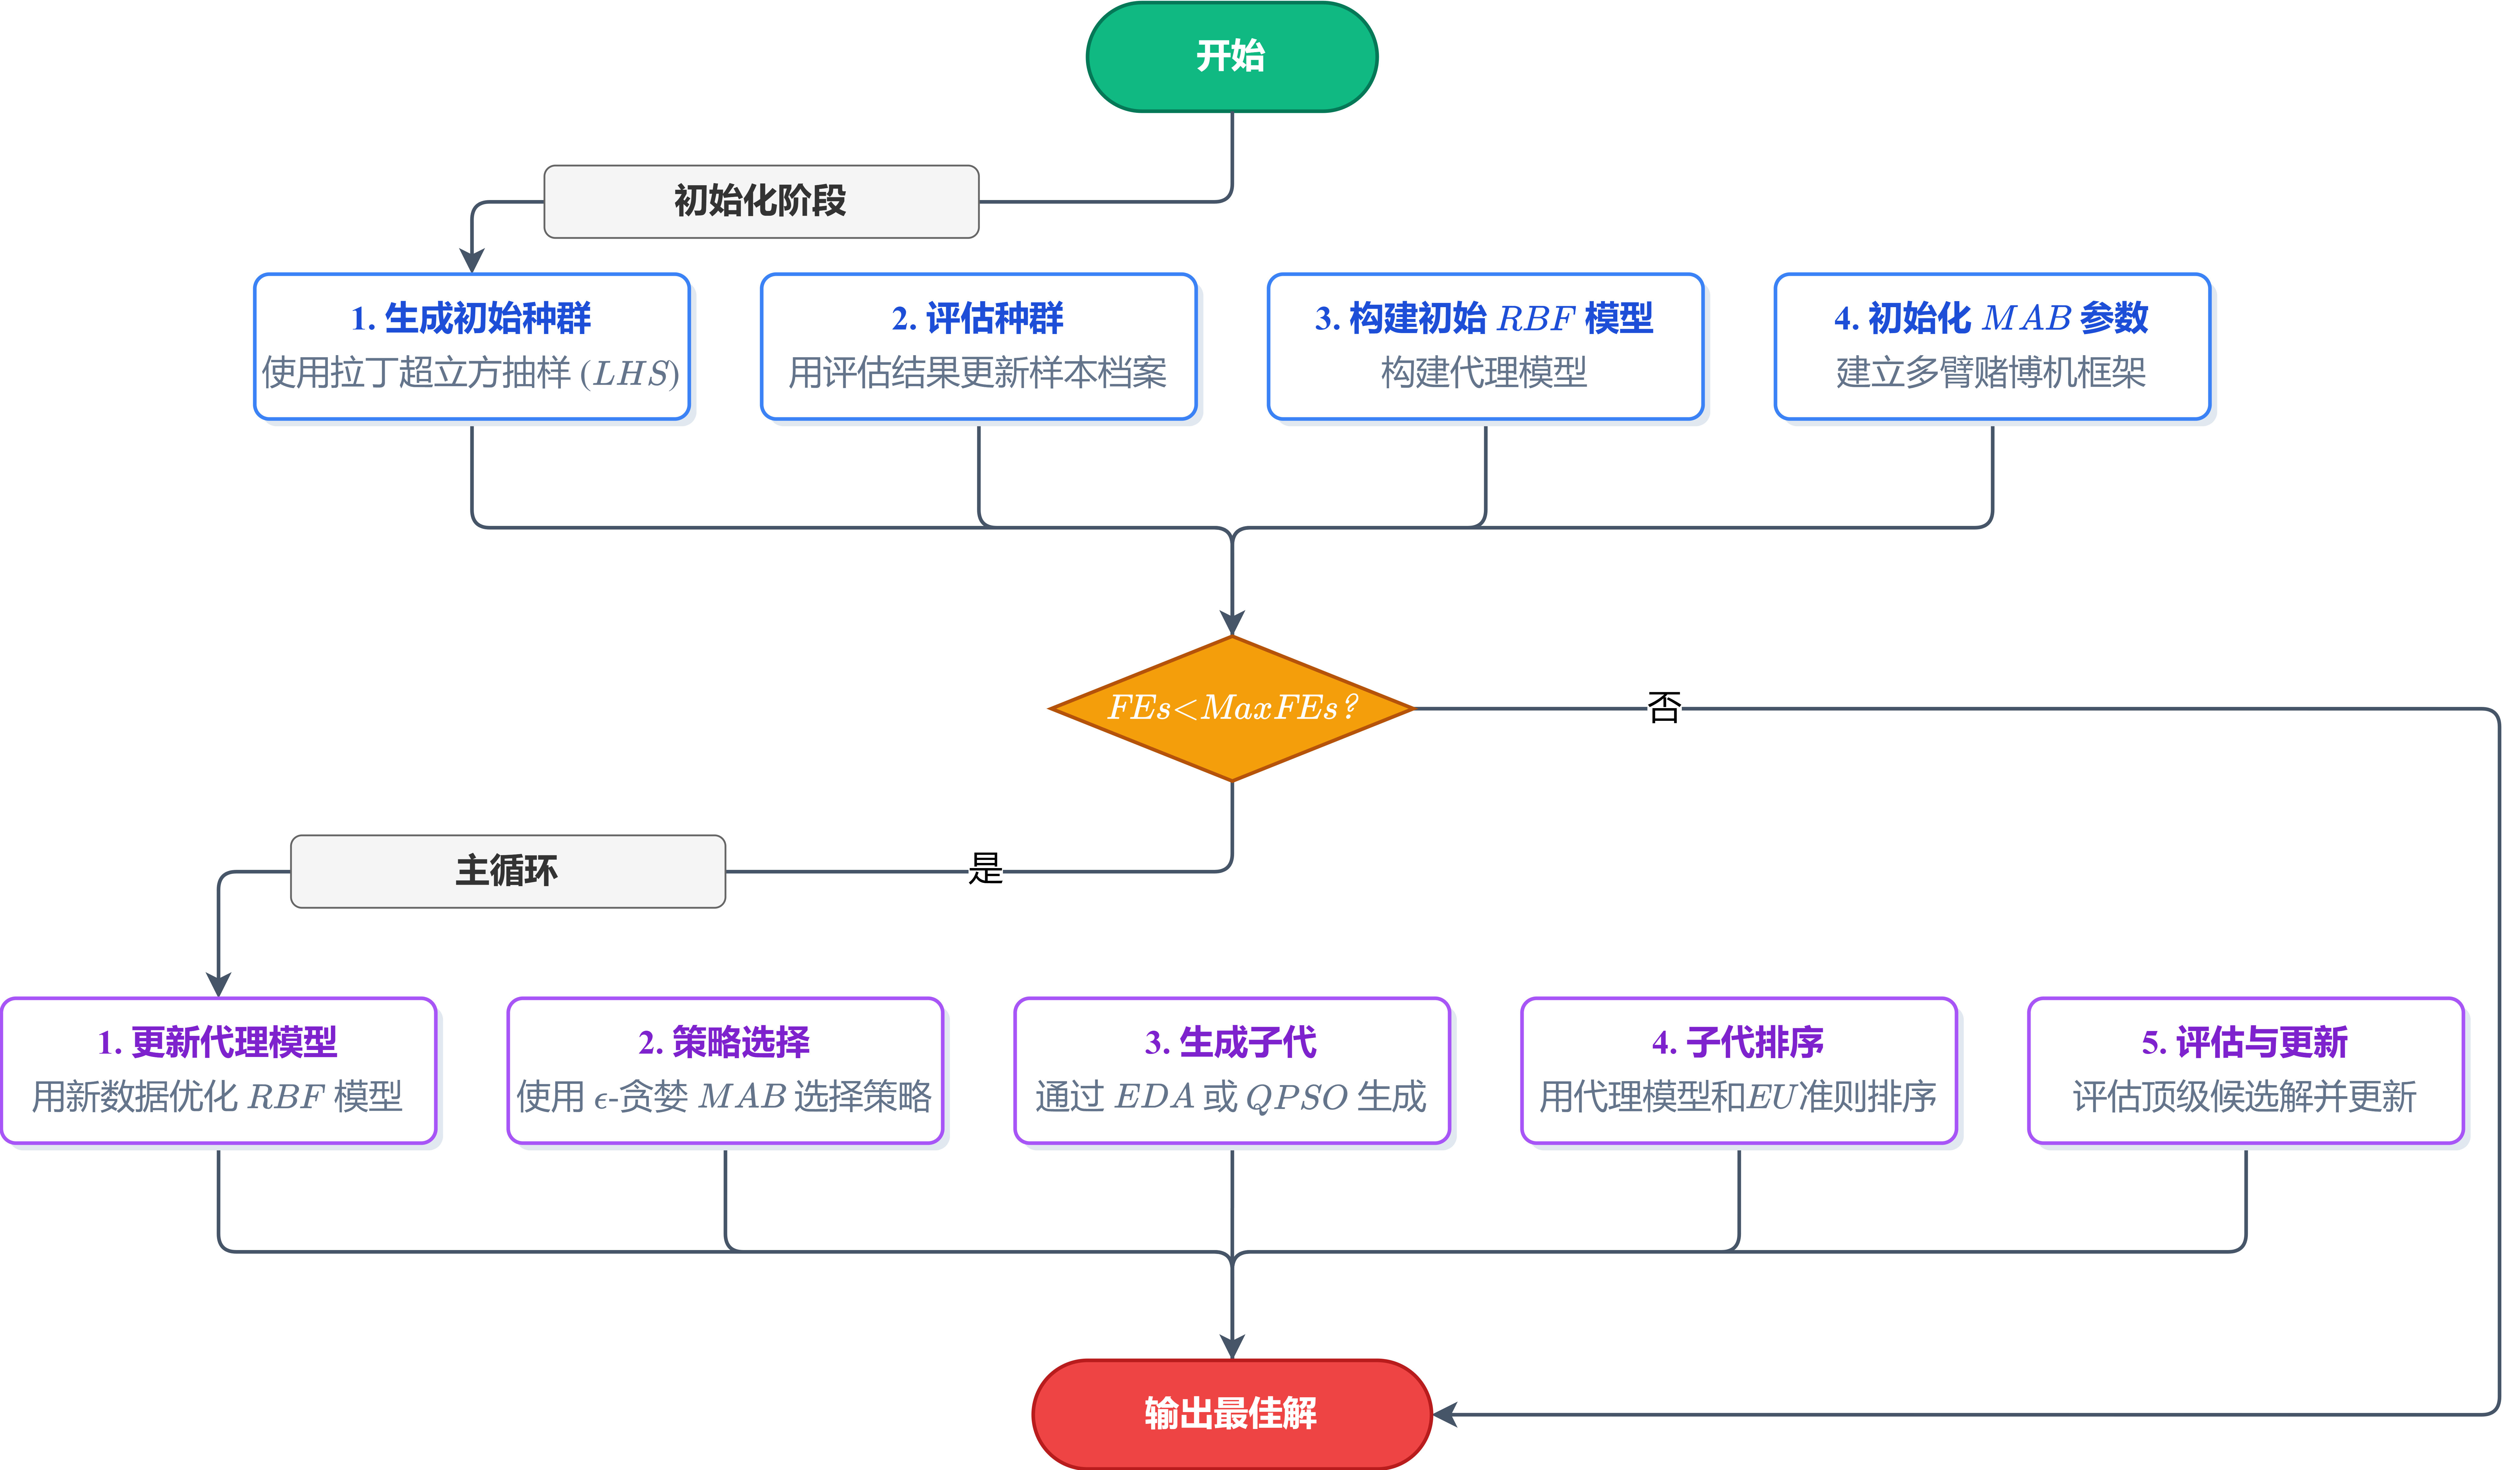
\includegraphics[width=\linewidth]{figures/chapter5/BEXEAStructure.png}
    \bicaption{BEXEA算法流程图}{Flowchart of the BEXEA algorithm}
    \label{fig:bexea_BEXEA}
\end{figure}

\subsection{多臂赌博机驱动的自适应搜索}
在线策略选择机制已被证明能够根据优化过程中的即时反馈，比静态分配更有效地平衡探索与开发\cite{xie2023surrogate,gong2024surrogate}。通过将$\epsilon$-贪心MAB嵌入SAEA，本章实现了EDA与QPSO策略的在线切换，并辅以停滞检测机制以增强算法的跳出能力。

具体实现中，策略选择被抽象为二臂赌博机问题。在每次迭代周期内，算法根据策略评分和探索概率选择执行动作。在获得新解的评估结果后，计算即时奖励并更新对应策略的价值估计$Q(a)$。

本章采用的$\epsilon$-贪心选择逻辑如下：
\begin{equation}
a_t =
\begin{cases}
\argmax\limits_a Q_t(a) & \text{with probability } 1-\epsilon \\
\text{random strategy} & \text{with probability } \epsilon
\end{cases}
\end{equation}
其中$\epsilon$设在0.1至0.3之间，通过维持适度的探索行为，防止算法过早陷入特定策略。

奖励函数的设计不仅考虑了适应度值的直接改进量，还结合了策略特有的贡献。例如在EDA阶段，会额外奖励能够提升种群多样性的搜索行为；而在QPSO阶段，则将解的可解释性评分纳入考量。这种多准则奖励机制使得算法能更精准地识别不同策略在特定搜索阶段的价值。

为了兼顾历史表现与近期收益，价值更新采用了指数近因加权平均。当搜索进程遭遇停滞（即连续若干次迭代未发现更优解）时，算法会主动上调探索率，强制尝试非贪心策略，从而提升全局搜索的活力。相比传统固定参数，这种动态调节策略更契合复杂优化问题在不同阶段对搜索力度的需求变化。

图\ref{fig:bexea_MAB}刻画了这一自适应过程。从初始化零评分开始，算法通过不断循环的“决策-评估-反馈”链条，自动演化出契合当前搜索景观的执行模式，在收敛效率与解的质量之间寻求最佳平衡。

\begin{figure}[ht]
    \centering
    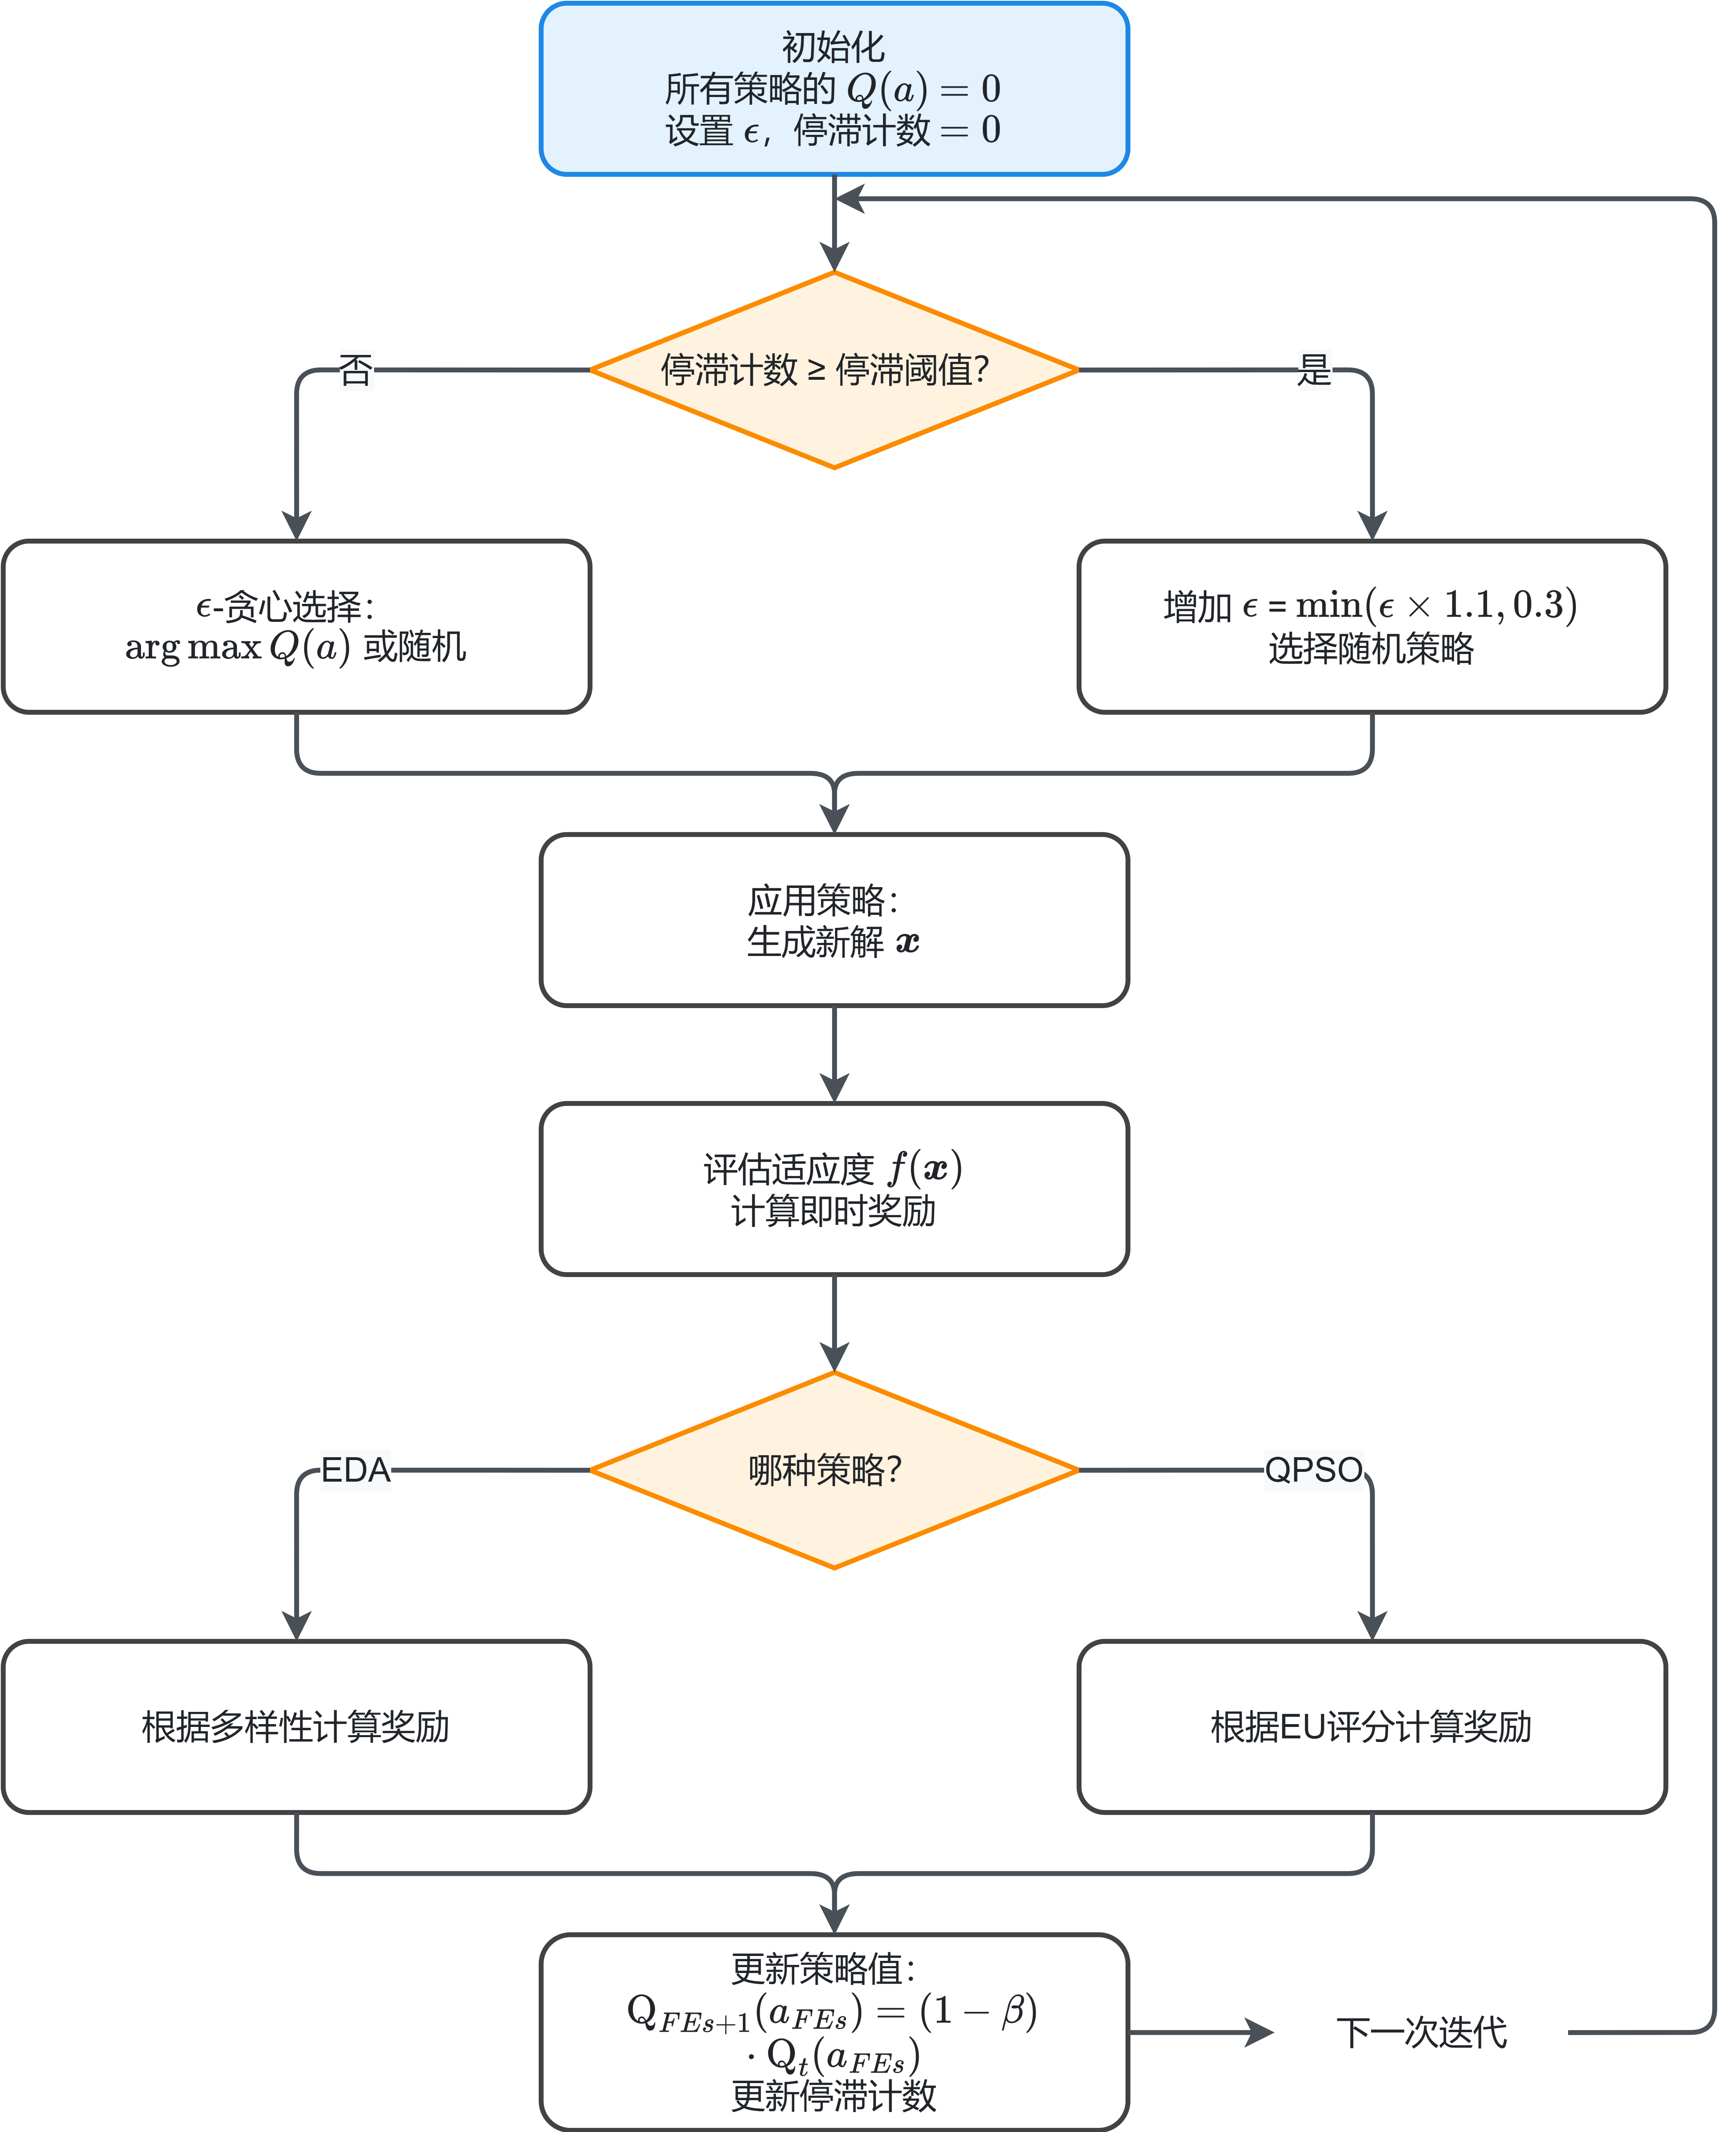
\includegraphics[width=\linewidth]{figures/chapter5/BEXEA-MAB.png}
    \bicaption{BEXEA中多臂赌博机驱动的自适应搜索}{Multi-armed bandit-driven adaptive search in BEXEA}
    \label{fig:bexea_MAB}
\end{figure}

\subsection{可解释不确定性准则}
EU准则融合了贝叶斯优化理论与可解释人工智能的思想，为采样决策提供了一套兼顾预测增量与决策透明度的衡量标准。

对于任一候选解，算法首先在历史档案中选取$\mathcal{K}$个近邻，基于局部数据估计其均值与标准差，进而计算期望改进（EI）。这一过程保证了采样对潜在最优区域的偏好。与此同时，本章创新性地计算了候选解相对于近邻的特征差异分布。受SHAP原理启发，这些差异被视为局部维度的重要性表征。

通过计算特征重要性分布的Shannon熵，可以量化预测判断背后的归因不确定性。高熵值通常意味着该点的预测驱动因素较为模糊，而低熵点则表明其具有更明确的归因依据。

最终形成的EU评价值将EI与反向的熵值相结合，使其表现出独特的优选逻辑：优先选择那些既具有显著改进潜力、又能够被清晰解释的候选区域。这种采样策略不仅有助于提升搜索的针对性，也为后续的工程决策提供了更扎实的可信度。在BEXEA中，EU准则不仅用于候选解的排序筛选，还作为赌博机奖励机制的关键组成部分，引导搜索策略向更具解释力的方向演化。

\begin{figure}[ht]
    \centering
    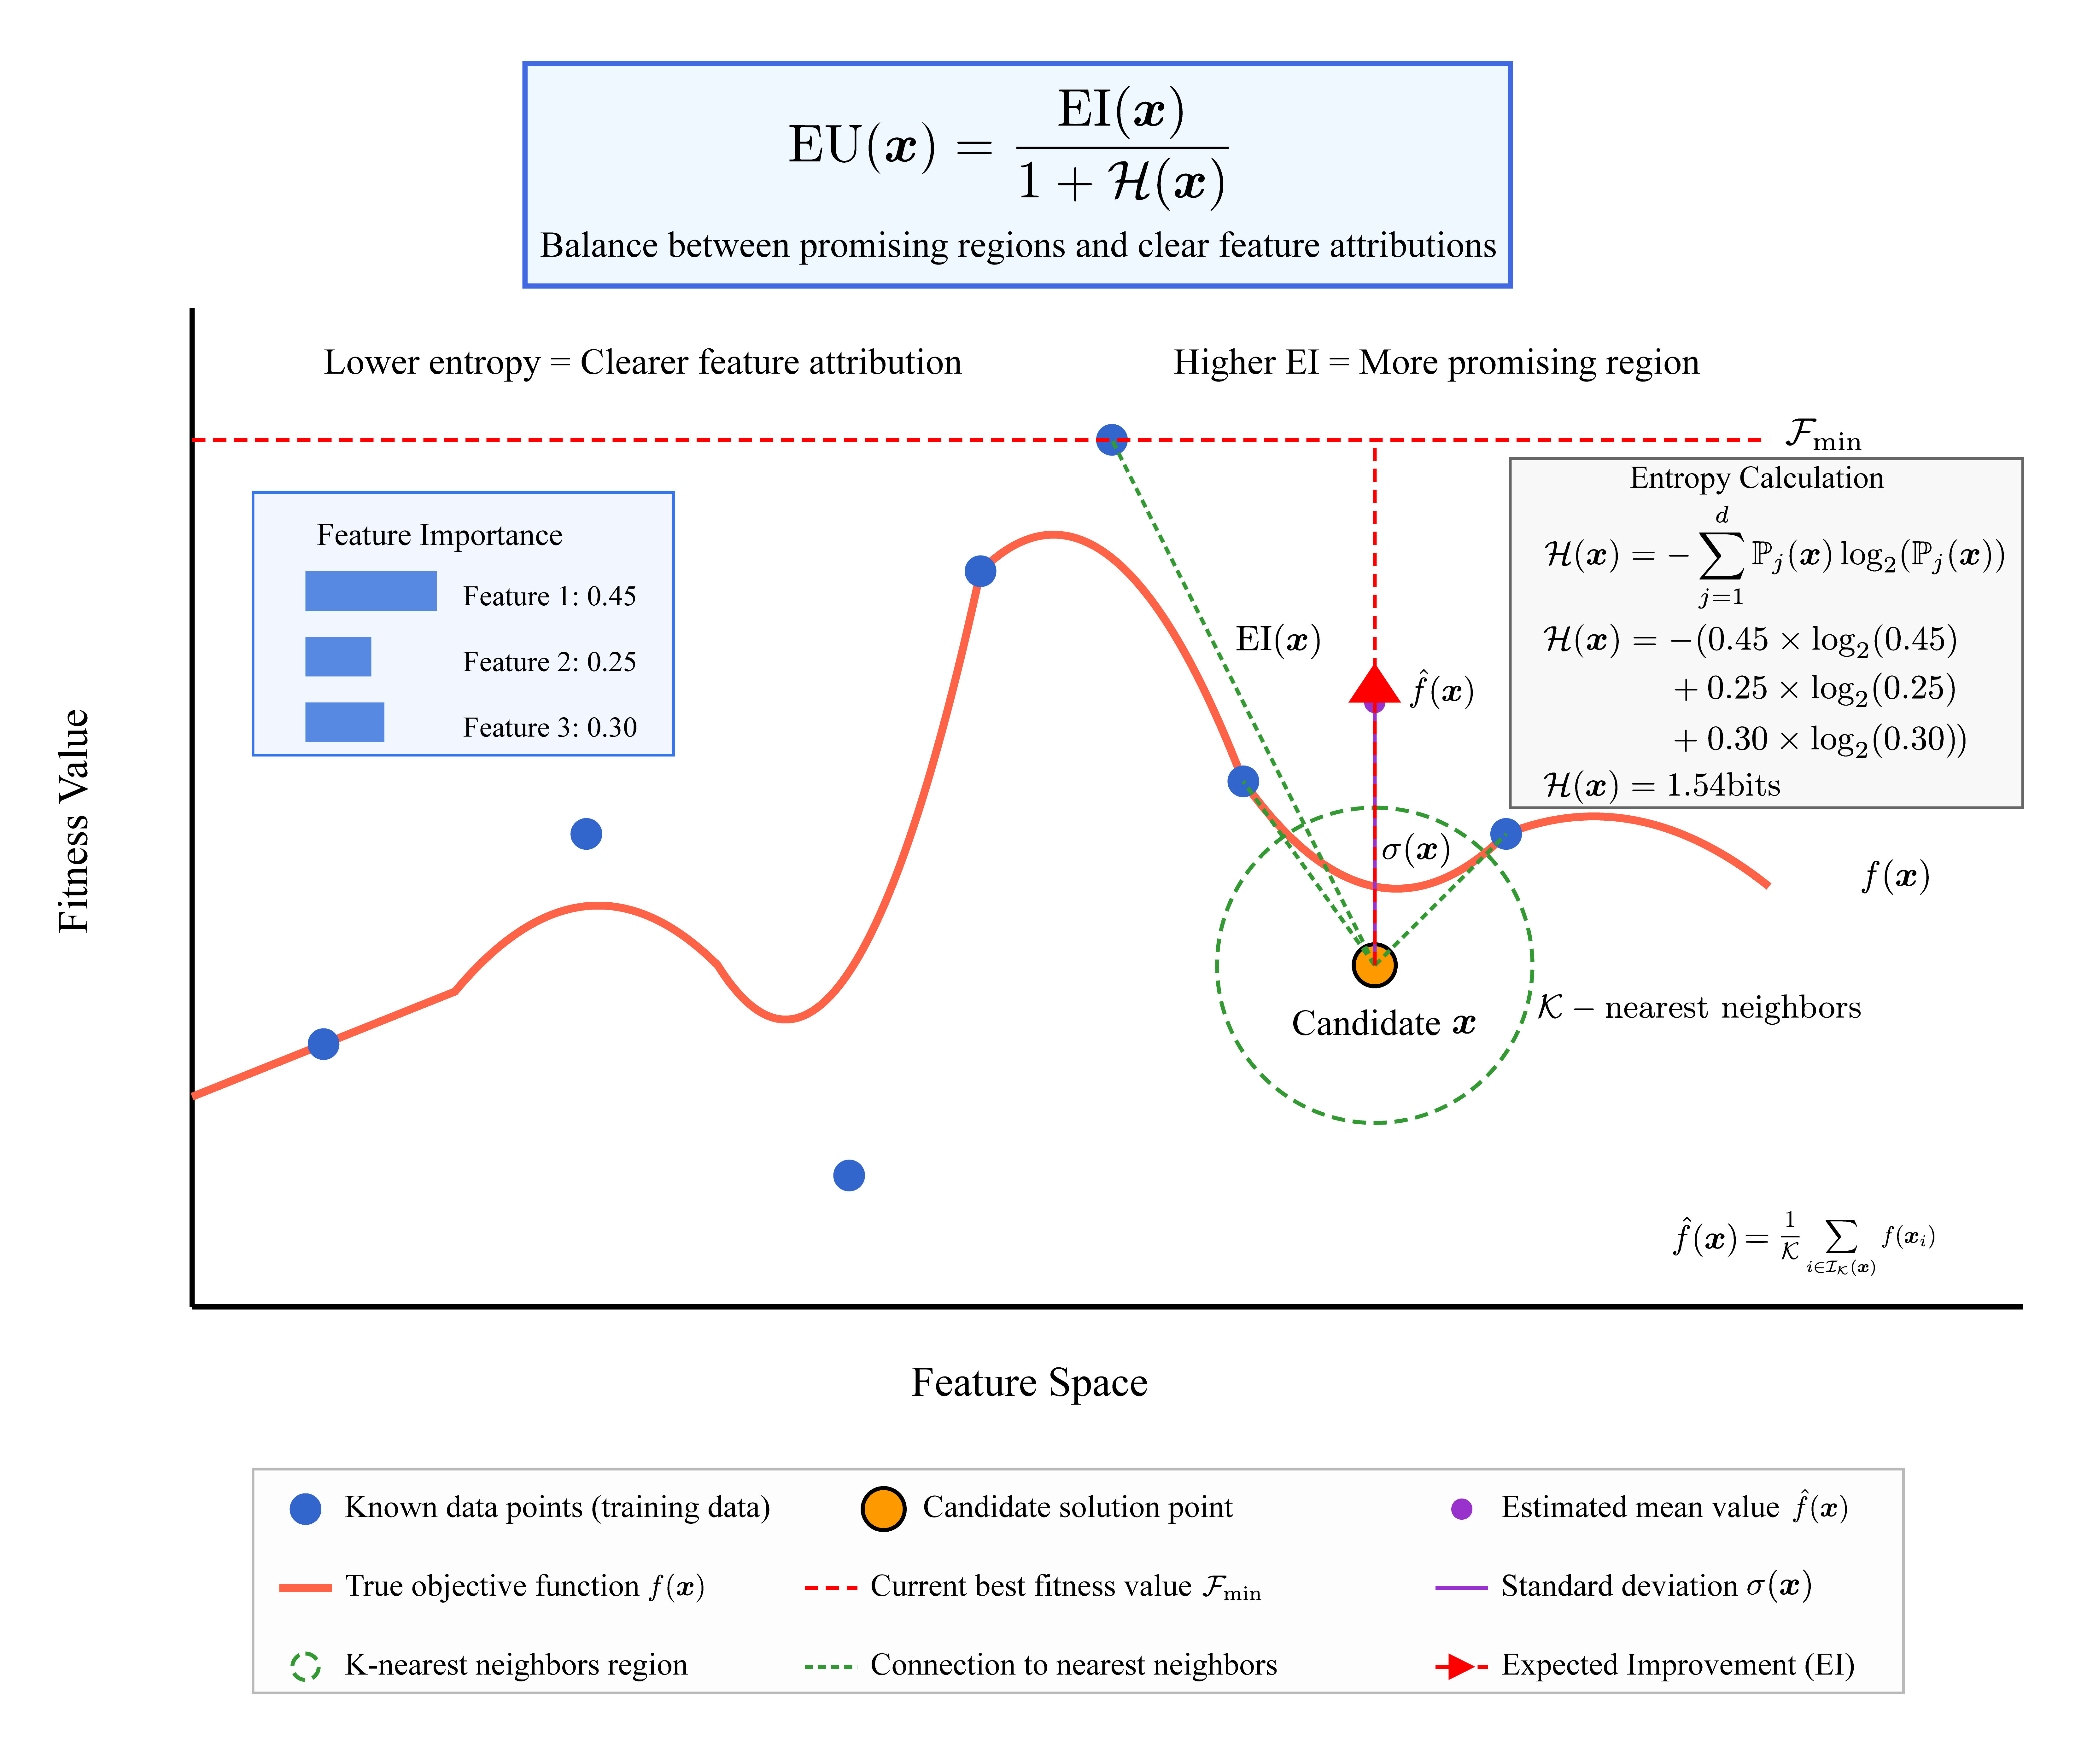
\includegraphics[width=\linewidth]{figures/chapter5/explainable-uncertainty-criteria-legend.png}
    \bicaption{可解释不确定性准则在三维函数上的示意图}{Illustration of the explainable uncertainty criteria on a 3-dimensional function}
    \label{fig:bexea_EU}
\end{figure}

\section{BEXEA的实验研究}

本节首先通过昂贵优化基准问题评估BEXEA的综合性能，随后将其应用于油藏产量优化算例，最后借助消融与参数实验对算法的核心机制进行深入解构。

\subsection{实验设置}

本研究采用了两组各具代表性的基准测试。首先是IEEE CEC 2022测试集（$d=20$），用于考察算法在标准维度下的优化能力。其次是针对高维场景设计的测试套件（$d=50$和$d=100$），涵盖了从简单单峰到复杂多峰旋转、混合等多种函数类型。实验数据的统计分析遵循第二章所述流程，统一采用Friedman检验与Wilcoxon秩和检验（置信水平$\alpha=0.05$），以确保对比结论的可靠性。

在竞争算法的选择上，本章挑选了TSA-BFEA、KTA2、DESO等七种具有代表性的先进SAEAs。为保证对比的公平性，所有算法的参数均严格执行原作者的推荐设置。BEXEA自身的衰减因子和近邻数分别固定为0.3和8。在所有测试任务中，函数评估上限设为1000次，每项测试均独立运行20次。

\subsection{油藏问题描述}

为了评估算法在工程实战中的表现，本章将其引入油藏产量优化任务中。该问题的核心是寻找最优的井控方案，以在权衡注水与生产成本后实现净现值（NPV）的最大化。

在本项研究中，采用经典的Egg模型进行测试。该系统包含8口注水井与4口生产井，构成了一个40维的决策空间。由于单次油藏模拟涉及到多相流偏微分方程的求解，计算代价极高。在这类真实昂贵场景下，算法被要求在仅有的200次评估预算内找到尽可能优的控制方案，这对其样本利用效率提出了极为苛刻的要求。

\begin{figure}[htbp]
    \centering
    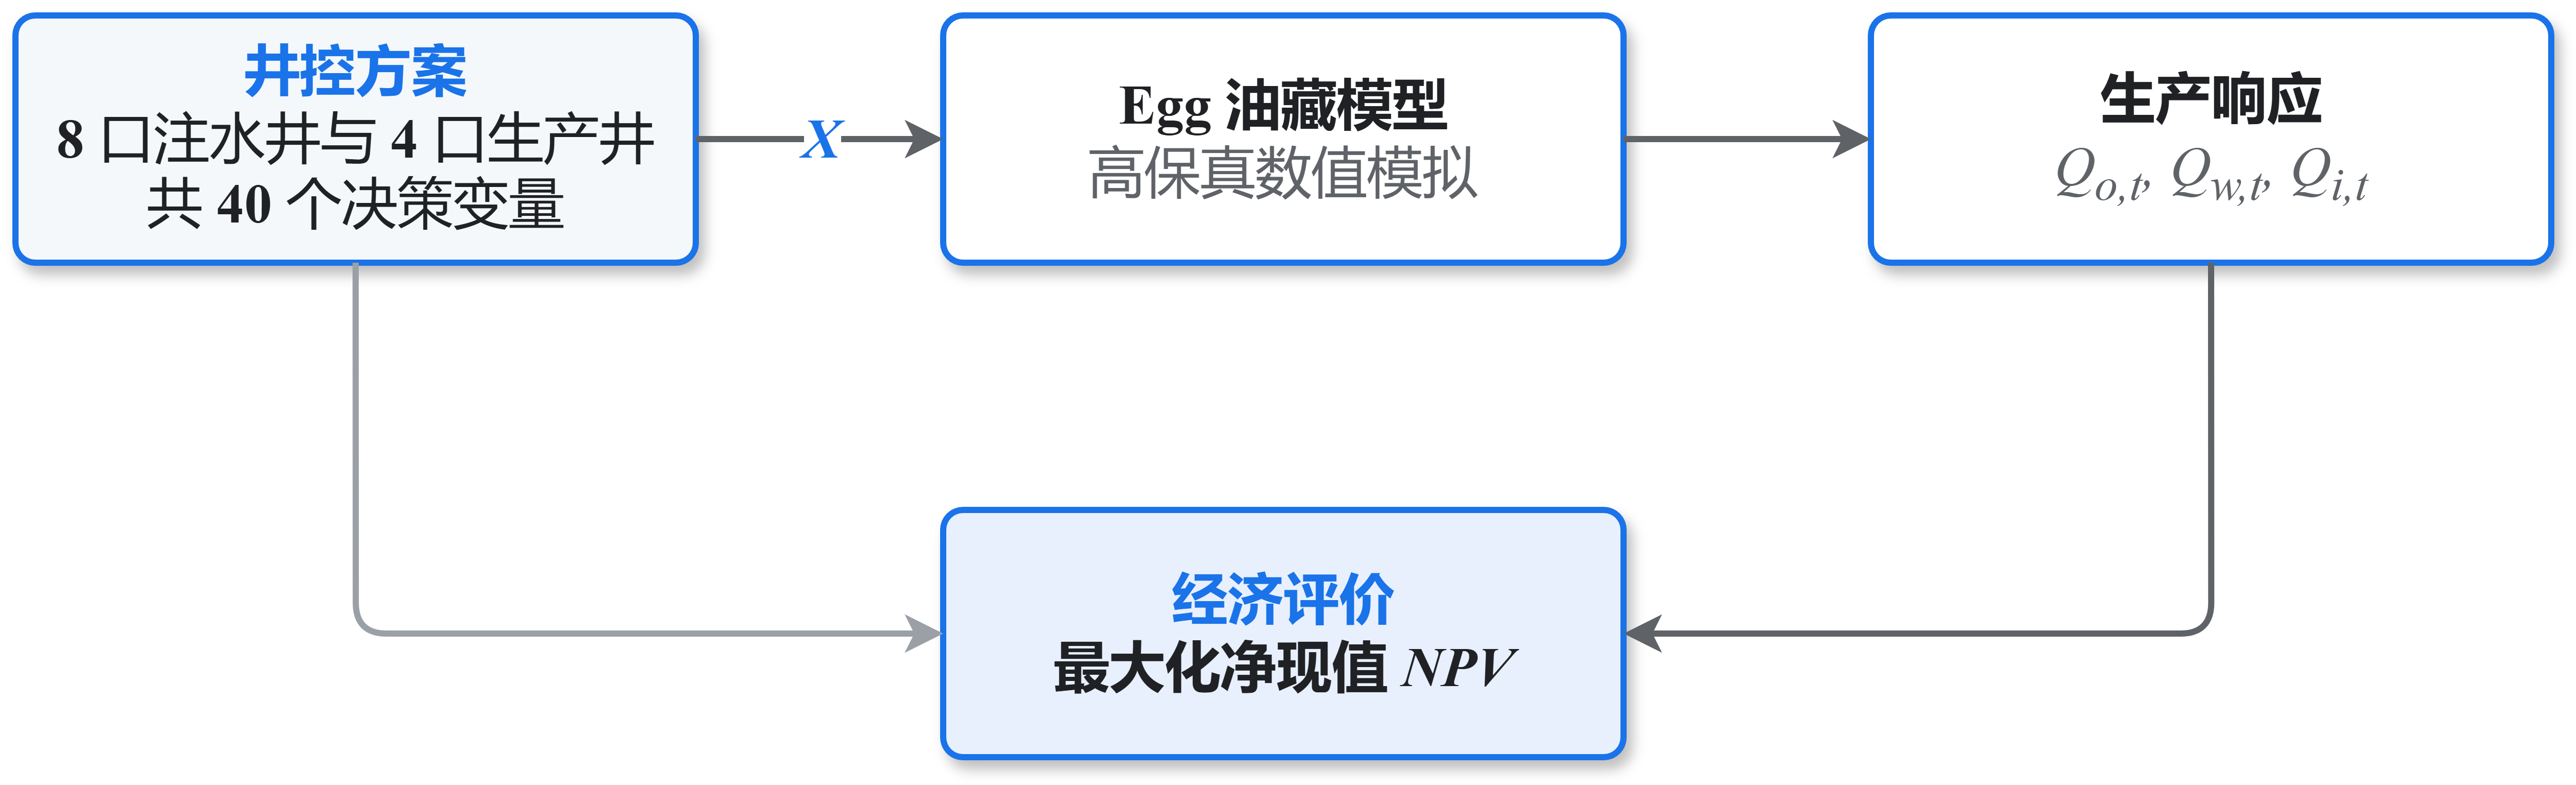
\includegraphics[width=0.86\textwidth]{figures/chapter5/BEXEA_application_workflow_refined.drawio.png}
    \bicaption{油藏产量优化问题示意图}{Schematic of the oil reservoir production optimization problem}
    \label{fig:bexea_oil_problem}
\end{figure}

如图\ref{fig:bexea_oil_problem}所示，井控决策方案经过高保真模拟器处理，输出产量数据，最终由经济模型折算为NPV。整个流程充分体现了昂贵优化问题中高开销、强非线性以及时空高度耦合的复杂特性。

\subsection{实验结果与分析}

本节将逐一分析BEXEA在基础函数测试与工程算例中的表现。

\subsubsection{昂贵优化基准实验}

表\ref{t:bexea_CEC22_Table}与表\ref{t:bexea_CEC05_Table}呈现了详细的对比数据。

\begin{table}[htbp]
\centering
\bicaption{BEXEA与竞争算法在IEEE CEC 2022测试套件上的比较结果（$d=20$）}{Comparison result of BEXEA and its competitors on IEEE CEC 2022 test suite with $d=20$}
\label{t:bexea_CEC22_Table}
\resizebox{\textwidth}{!}{\begin{tabular}{lccccc}
\toprule
Problem & TSA-BFEA & KTA2 & DESO & MS-MTO & BEXEA \\
\midrule
F1 & 5.933E+04(1.38E+04)= & 2.836E+06(8.60E+06)= & 6.914E+04(1.44E+04)= & 7.342E+04(1.76E+04)= & {5.349E+04(1.70E+04)} \\
F2 & 1.778E+03(3.53E+02)= & 2.717E+03(3.24E+03)+ & 2.464E+03(6.82E+02)+ & 3.040E+03(7.88E+02)+ & \textbf{4.536E+02(8.78E+00)} \\
F3 & 6.720E+02(9.72E+00)+ & 6.769E+02(3.97E+01)+ & 6.746E+02(1.46E+01)+ & 6.993E+02(9.61E+00)+ & \textbf{6.118E+02(1.11E+01)} \\
F4 & 9.915E+02(1.83E+01)+ & 9.980E+02(7.02E+01)+ & 9.828E+02(2.67E+01)+ & 1.064E+03(3.46E+01)+ & \textbf{8.363E+02(1.14E+01)} \\
F5 & 5.072E+03(6.50E+02)+ & 6.314E+03(5.22E+03)+ & 4.401E+03(1.33E+03)+ & 9.870E+03(2.43E+03)+ & \textbf{1.094E+03(2.06E+02)} \\
F6 & 1.418E+09(7.00E+08)+ & 1.484E+09(2.16E+09)+ & 1.297E+09(6.03E+08)+ & 4.444E+09(1.53E+09)+ & \textbf{3.665E+03(1.46E+03)} \\
F7 & 2.253E+03(5.94E+01)+ & 2.422E+03(1.51E+02)+ & 2.270E+03(7.88E+01)+ & 2.469E+03(1.18E+02)+ & \textbf{2.127E+03(7.97E+01)} \\
F8 & 2.767E+03(2.62E+02)+ & 3.011E+03(4.58E+02)+ & 2.450E+03(1.20E+02)+ & 2.787E+03(1.23E+02)+ & \textbf{2.279E+03(5.88E+01)} \\
F9 & 2.970E+03(1.04E+02)+ & 3.011E+03(5.97E+02)+ & 3.231E+03(2.91E+02)+ & 3.298E+03(1.96E+02)+ & \textbf{2.496E+03(1.55E+01)} \\
F10 & 5.217E+03(2.05E+03)+ & 6.669E+03(1.93E+03)+ & 6.120E+03(1.96E+03)+ & 8.185E+03(5.66E+02)+ & \textbf{3.558E+03(1.12E+03)} \\
F11 & 8.254E+03(7.23E+02)+ & 9.330E+03(3.76E+03)+ & 8.174E+03(7.03E+02)+ & 9.234E+03(1.08E+03)+ & \textbf{2.902E+03(6.16E-01)} \\
F12 & 3.488E+03(1.43E+02)+ & 3.814E+03(4.00E+02)+ & 3.991E+03(1.93E+02)+ & 3.642E+03(1.54E+02)+ & \textbf{3.006E+03(3.70E+01)} \\
\midrule
Ranking & 4.2 & 6.3 & 4.5 & 6.8 & \textbf{1.1} \\
+/-/= & 10/0/2 & 11/0/1 & 11/0/1 & 11/0/1 & NA \\
\bottomrule
\end{tabular}}

\vspace{4pt}
\resizebox{\textwidth}{!}{\begin{tabular}{lcccc}
\toprule
Problem & ESA & eToSADE & SHPSO & BEXEA \\
\midrule
F1 & 7.466E+04(2.64E+04)= & \textbf{5.206E+04(1.10E+04)=} & 5.470E+04(1.52E+04)= & {5.349E+04(1.70E+04)} \\
F2 & 7.269E+03(1.78E+03)+ & 1.441E+03(3.16E+02)= & 4.944E+02(2.15E+01)= & \textbf{4.536E+02(8.78E+00)} \\
F3 & 7.015E+02(8.62E+00)+ & 6.689E+02(1.01E+01)+ & 6.239E+02(5.83E+00)+ & \textbf{6.118E+02(1.11E+01)} \\
F4 & 1.070E+03(2.02E+01)+ & 9.944E+02(1.13E+01)+ & 9.428E+02(1.55E+01)+ & \textbf{8.363E+02(1.14E+01)} \\
F5 & 9.096E+03(1.20E+03)+ & 5.360E+03(9.01E+02)+ & 1.264E+03(2.60E+02)+ & \textbf{1.094E+03(2.06E+02)} \\
F6 & 6.796E+09(2.12E+09)+ & 7.825E+08(3.00E+08)+ & 4.465E+07(2.12E+07)= & \textbf{3.665E+03(1.46E+03)} \\
F7 & 2.365E+03(8.57E+01)+ & 2.297E+03(6.38E+01)+ & 2.213E+03(6.14E+01)+ & \textbf{2.127E+03(7.97E+01)} \\
F8 & 4.136E+03(2.50E+03)+ & 2.456E+03(9.63E+01)+ & 2.313E+03(6.43E+01)+ & \textbf{2.279E+03(5.88E+01)} \\
F9 & 3.819E+03(4.30E+02)+ & 2.771E+03(5.97E+01)+ & 2.572E+03(3.68E+01)= & \textbf{2.496E+03(1.55E+01)} \\
F10 & 7.003E+03(1.20E+03)+ & 4.280E+03(1.79E+03)+ & 5.182E+03(2.24E+03)+ & \textbf{3.558E+03(1.12E+03)} \\
F11 & 1.299E+04(1.96E+03)+ & 6.569E+03(7.16E+02)= & 3.331E+03(9.54E+01)+ & \textbf{2.902E+03(6.16E-01)} \\
F12 & 4.062E+03(1.78E+02)+ & 3.180E+03(6.87E+01)+ & 3.032E+03(4.10E+01)+ & \textbf{3.006E+03(3.70E+01)} \\
\midrule
Ranking & 7.6 & 3.3 & 2.2 & \textbf{1.1} \\
+/-/= & 11/0/1 & 9/0/3 & 8/0/4 & NA \\
\bottomrule
\end{tabular}}
\end{table}

在IEEE CEC 2022测试中，BEXEA展现出了显著的竞争优势，Friedman平均排名稳居首位（1.1）。在Wilcoxon显著性检验中，绝大多数测试项均支持BEXEA占优。这种稳健的全局寻优能力主要归因于两个方面的协同：首先是MAB机制实现的策略动态平衡，它能依据搜索状态实时倾斜资源，避免了算法在某些阶段出现策略失配；其次是EU准则对评估预算的精准导向，它不仅追求数值上的改进，更侧重于归因清晰的优质区域，从而极大地提高了单次真实评估的含金量。

\begin{figure}
    \centering
    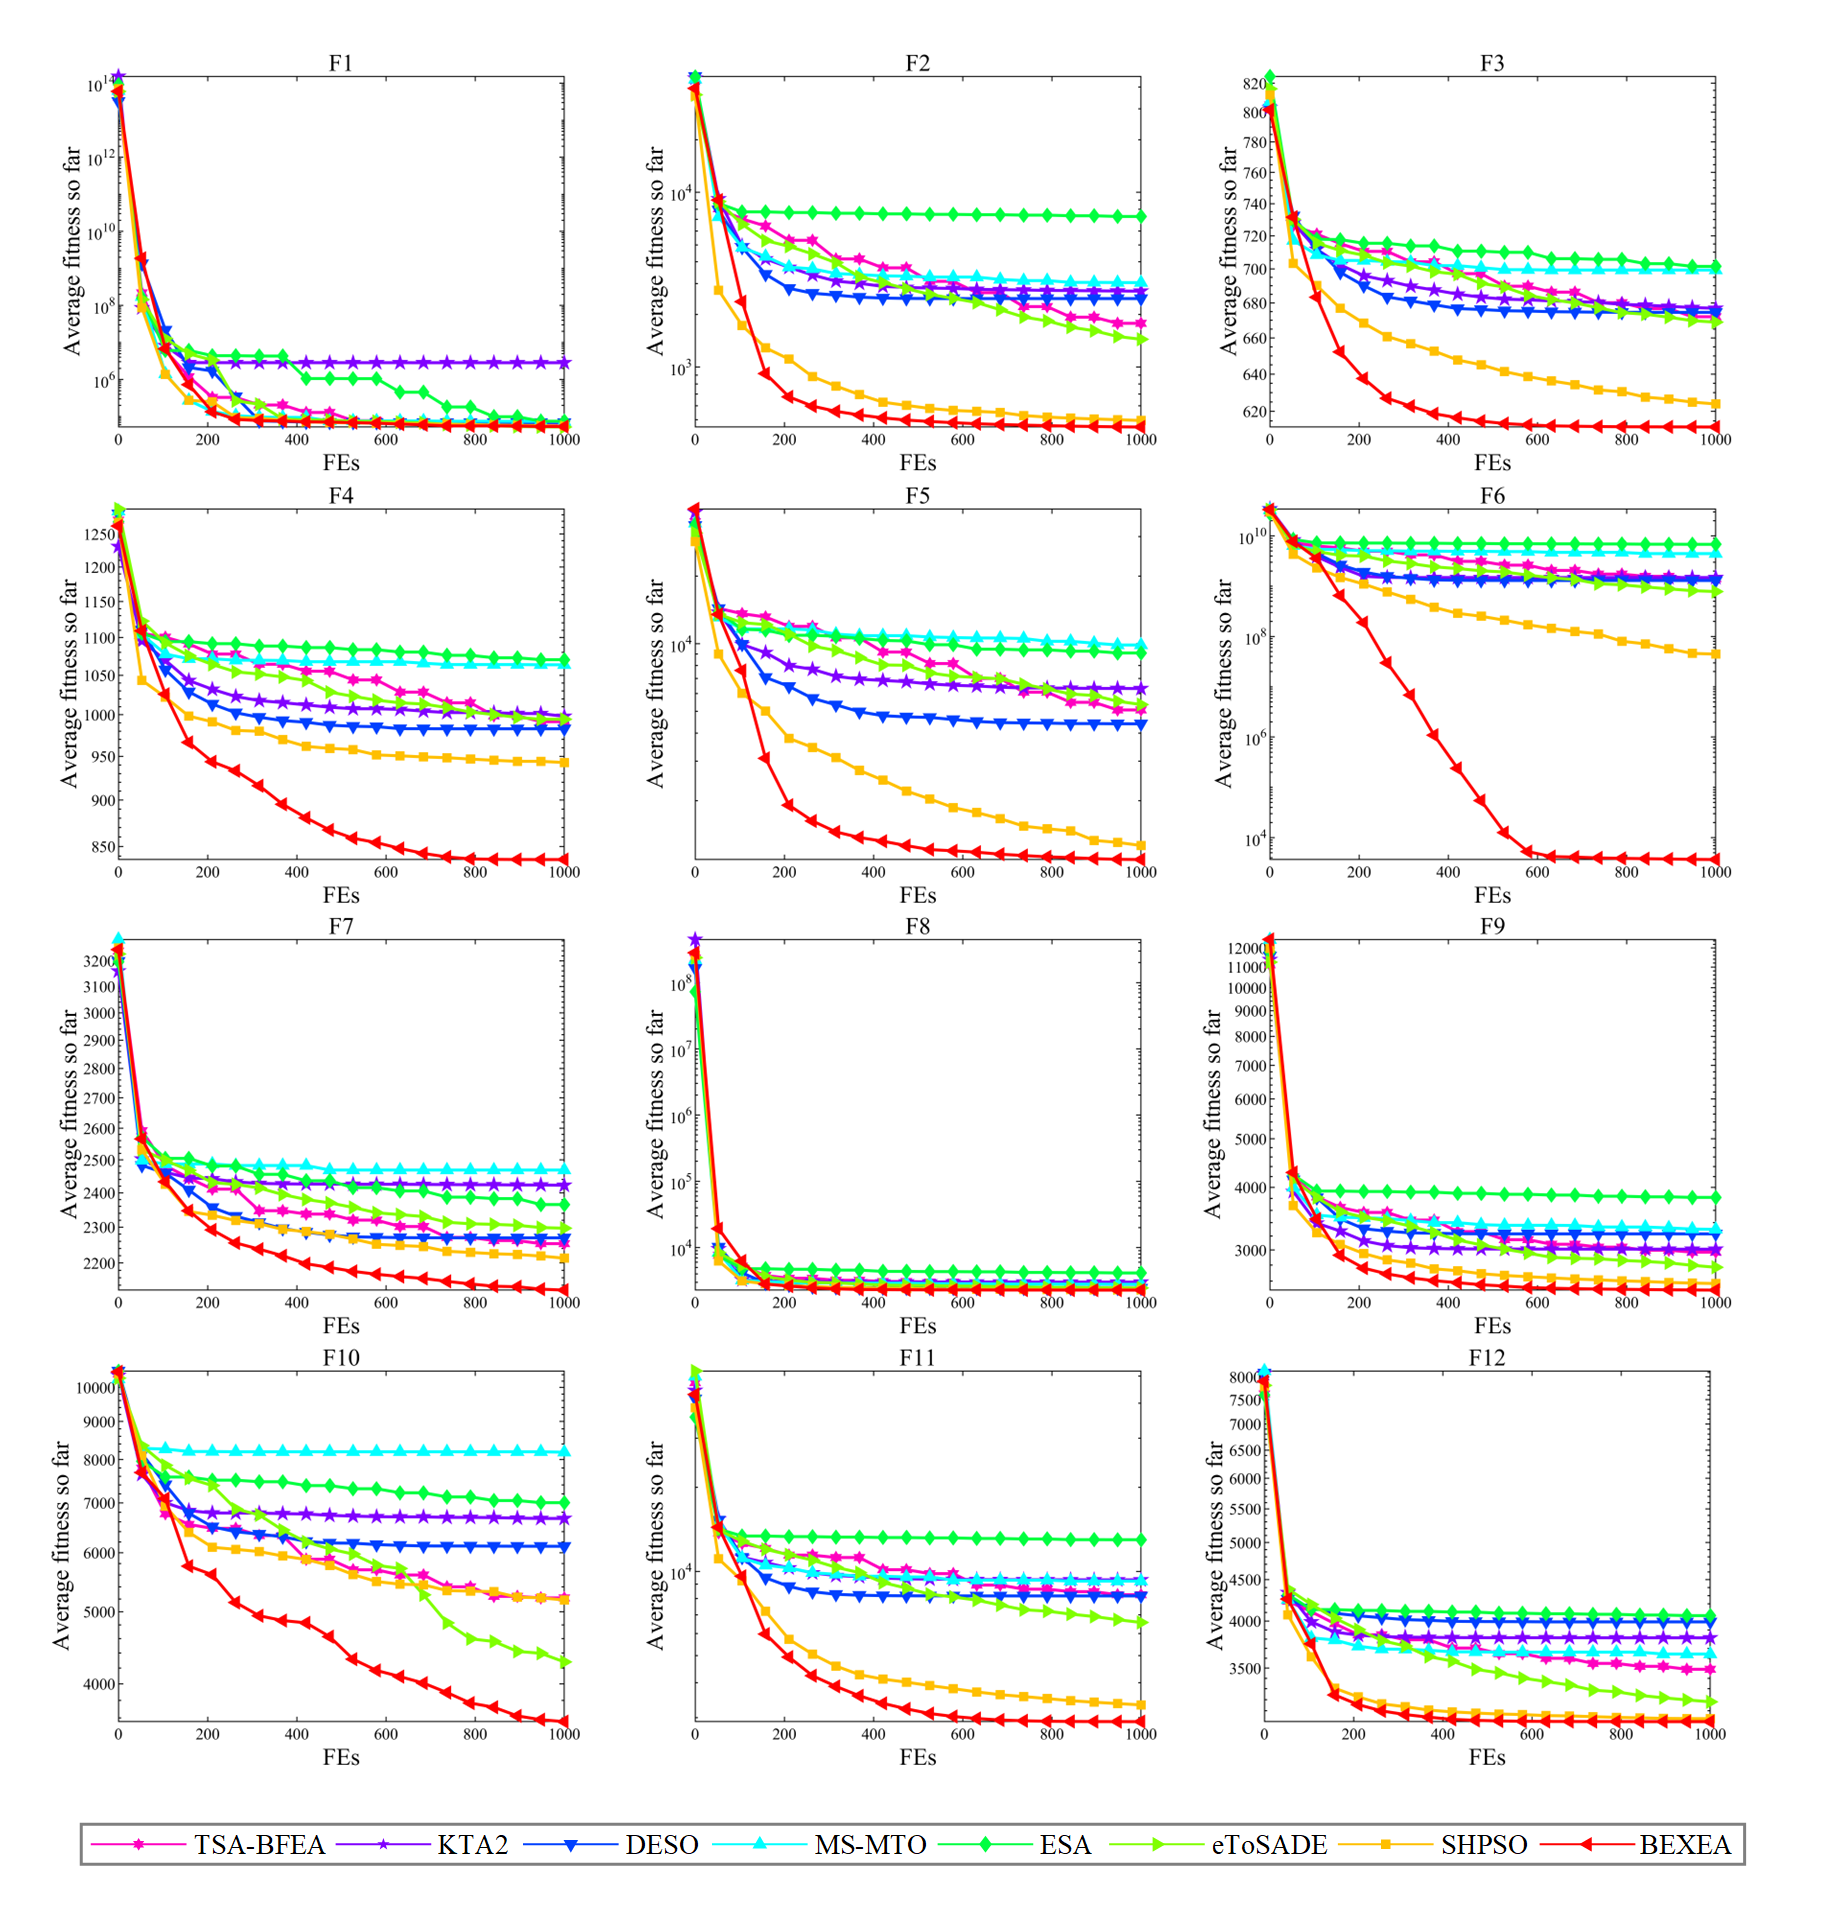
\includegraphics[width=\linewidth]{figures/chapter5/BEXEA-CEC22-CC.png}
    \bicaption{BEXEA与竞争算法在IEEE CEC 2022测试套件上的收敛曲线（$d=20$）}{Convergence curves of BEXEA and its competitors on the IEEE CEC 2022 test suite ($d=20$)}
    \label{fig:bexea_CEC22_CC}
\end{figure}

收敛曲线图\ref{fig:bexea_CEC22_CC}进一步印证了上述观点。在多个极具挑战性的函数（如F4、F6）上，BEXEA均能以更快的速度逼近更低的适应度值，体现了自适应搜索在调节探索与开发力度方面的灵活性。

此外，散点分布图\ref{fig:bexea_CEC22_Plots}显示BEXEA的运行结果更为集中，反映了该算法在不同随机种子下表现出的良好稳定性。

在高维测试场景中（表\ref{t:bexea_CEC05_Table}），BEXEA的优势依然显著。即便维度提升至100维，MAB驱动的策略切换依然能有效应对复杂的搜索景观。尤其是在面对多模态函数时，这种机制能有效维持搜索的多样性，降低陷入局部最优的风险。这充分证明了BEXEA在处理中高维优化任务时具有良好的可扩展性。

\begin{figure}
    \centering
    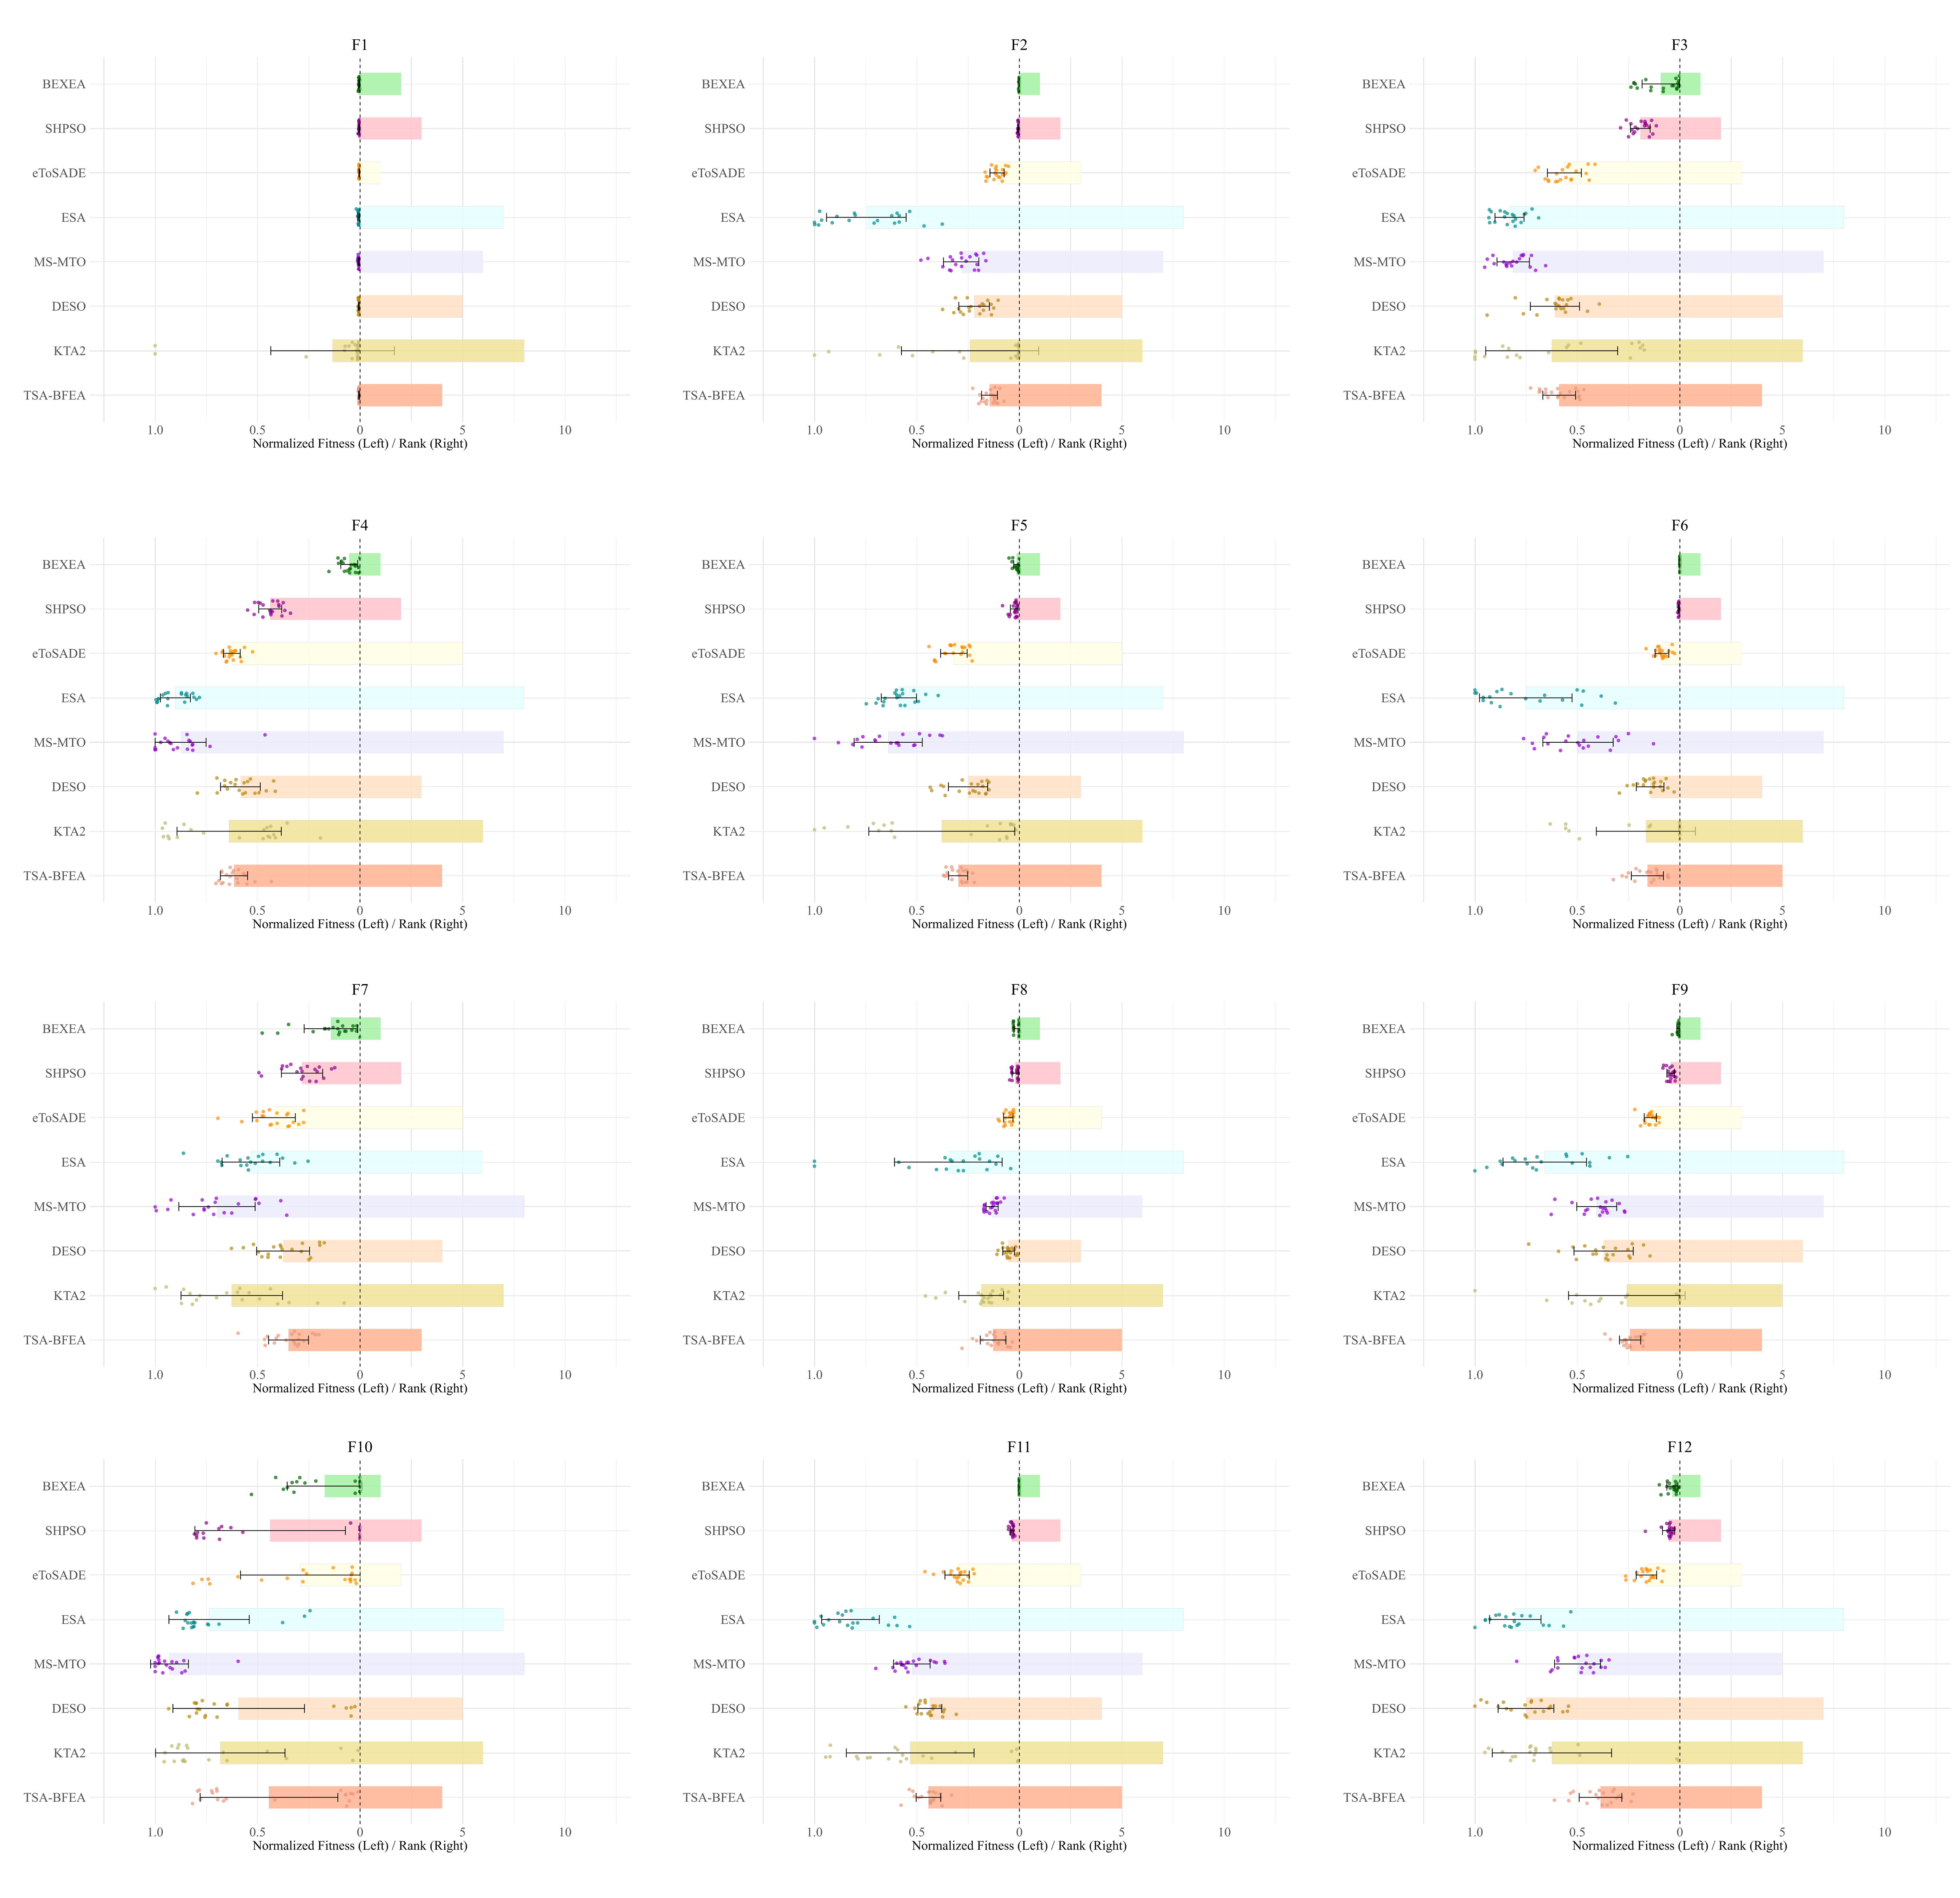
\includegraphics[width=\textwidth]{figures/chapter5/BEXEA-Plots.png}
    \bicaption{BEXEA与竞争算法在IEEE CEC 2022测试套件上的散点图和排名图（$d=20$）}{Combined scatter and rank plots of BEXEA and its competitors on the IEEE CEC 2022 test suite ($d=20$)}
    \label{fig:bexea_CEC22_Plots}
\end{figure}

\begin{table}[htbp]
\centering
\bicaption{BEXEA与竞争算法在昂贵函数测试套件上的比较结果（$d=50$和$d=100$）}{Comparison results of BEXEA and its competitors on the expensive functions test suite with $d=50$ and $d=100$}
\label{t:bexea_CEC05_Table}
\resizebox{\textwidth}{!}{\begin{tabular}{lccccc}
\toprule
Problem & TSA-BFEA & KTA2 & DESO & MS-MTO & BEXEA \\
\midrule
ELLIPSOID-50D & 3.739E+03(3.91E+02)= & 4.084E+03(1.61E+03)= & 1.668E+03(2.36E+02)= & 6.138E+03(7.88E+02)= & \textbf{3.804E+00(1.30E+01)} \\
ELLIPSOID-100D & 2.275E+04(1.98E+03)= & 2.166E+04(6.24E+03)= & 8.687E+03(8.92E+02)= & 3.153E+04(1.45E+03)= & \textbf{3.761E+02(2.63E+02)} \\
ROSENBROCK-50D & 5.220E+03(6.50E+02)+ & 7.696E+03(3.31E+03)+ & 1.681E+03(2.64E+02)+ & 1.003E+04(8.12E+02)+ & \textbf{6.395E+01(3.13E+01)} \\
ROSENBROCK-100D & 1.879E+04(1.76E+03)+ & 1.697E+04(6.02E+03)+ & 4.554E+03(5.54E+02)+ & 2.829E+04(2.75E+03)+ & \textbf{3.355E+02(1.46E+02)} \\
ACKLEY-50D & 1.971E+01(1.32E-01)+ & 2.002E+01(5.83E-01)+ & 1.743E+01(4.96E-01)+ & 2.060E+01(7.61E-02)+ & \textbf{6.695E+00(4.88E+00)} \\
ACKLEY-100D & 2.080E+01(8.07E-02)+ & 2.013E+01(3.05E-01)+ & 1.808E+01(3.29E-01)+ & 2.075E+01(6.40E-02)+ & \textbf{8.868E+00(3.90E+00)} \\
GRIEWANK-50D & 5.739E+02(4.64E+01)+ & 6.260E+02(1.41E+02)+ & 2.535E+02(2.83E+01)+ & 8.116E+02(4.43E+01)+ & 1.384E+01(2.59E+01) \\
GRIEWANK-100D & 1.618E+03(8.46E+01)+ & 1.644E+03(5.32E+02)+ & 6.231E+02(4.40E+01)+ & 2.010E+03(5.44E+01)+ & 8.889E+01(8.31E+01) \\
RASTRIGIN-50D & 5.850E+02(2.68E+01)+ & 6.576E+02(4.98E+01)+ & 4.825E+02(2.63E+01)+ & 7.101E+02(2.21E+01)+ & \textbf{1.108E+02(4.12E+01)} \\
RASTRIGIN-100D & 1.386E+03(5.11E+01)+ & 1.403E+03(1.14E+02)+ & 1.025E+03(4.68E+01)+ & 1.539E+03(3.76E+01)+ & \textbf{4.245E+02(9.07E+01)} \\
SRR-50D & 8.207E+02(7.65E+01)+ & 1.146E+03(1.77E+02)+ & 8.564E+02(6.92E+01)+ & 1.008E+03(6.47E+01)+ & \textbf{-4.131E+01(1.00E+02)} \\
SRR-100D & 2.407E+03(1.11E+02)+ & 2.663E+03(2.02E+02)+ & 1.982E+03(1.14E+02)+ & 2.377E+03(9.53E+01)+ & 1.260E+03(2.04E+02) \\
RHC-50D & 1.359E+03(2.87E+01)+ & 1.461E+03(4.52E+01)+ & 1.369E+03(2.47E+01)+ & 1.452E+03(4.18E+01)+ & 1.089E+03(5.83E+01) \\
RHC-100D & 1.504E+03(5.08E+01)+ & 1.500E+03(2.88E+01)+ & 1.421E+03(1.64E+01)+ & 1.504E+03(3.37E+01)+ & \textbf{1.389E+03(2.50E+01)} \\
\midrule
Ranking & 5.4 & 6.0 & 3.2 & 6.9 & \textbf{1.3} \\
+/-/= & 12/0/2 & 12/0/2 & 12/0/2 & 12/0/2 & NA \\
\bottomrule
\end{tabular}}

\vspace{4pt}
\resizebox{\textwidth}{!}{\begin{tabular}{lcccc}
\toprule
Problem & ESA & eToSADE & SHPSO & BEXEA \\
\midrule
ELLIPSOID-50D & 6.254E+03(4.97E+02)= & 2.752E+03(4.60E+02)= & 9.858E+01(2.42E+01)= & \textbf{3.804E+00(1.30E+01)} \\
ELLIPSOID-100D & 3.034E+04(1.06E+03)= & 1.414E+04(2.26E+03)= & 8.328E+02(1.27E+02)= & \textbf{3.761E+02(2.63E+02)} \\
ROSENBROCK-50D & 1.354E+04(1.17E+03)+ & 3.445E+03(9.42E+02)+ & 1.332E+02(2.22E+01)+ & \textbf{6.395E+01(3.13E+01)} \\
ROSENBROCK-100D & 3.211E+04(2.29E+03)+ & 9.911E+03(2.59E+03)+ & 4.845E+02(7.88E+01)+ & \textbf{3.355E+02(1.46E+02)} \\
ACKLEY-50D & 2.067E+01(8.21E-02)+ & 1.881E+01(6.39E-01)+ & 6.739E+00(6.60E-01)+ & \textbf{6.695E+00(4.88E+00)} \\
ACKLEY-100D & 2.088E+01(5.00E-02)+ & 1.933E+01(5.24E-01)+ & 9.558E+00(7.22E-01)+ & \textbf{8.868E+00(3.90E+00)} \\
GRIEWANK-50D & 1.046E+03(5.78E+01)+ & 4.218E+02(5.75E+01)+ & \textbf{6.268E+00(1.34E+00)=} & 1.384E+01(2.59E+01) \\
GRIEWANK-100D & 2.360E+03(9.14E+01)+ & 9.784E+02(1.70E+02)+ & \textbf{2.652E+01(3.48E+00)-} & 8.889E+01(8.31E+01) \\
RASTRIGIN-50D & 6.772E+02(2.09E+01)+ & 5.458E+02(2.99E+01)+ & 4.371E+02(3.59E+01)= & \textbf{1.108E+02(4.12E+01)} \\
RASTRIGIN-100D & 1.487E+03(3.63E+01)+ & 1.231E+03(5.63E+01)+ & 9.574E+02(6.81E+01)+ & \textbf{4.245E+02(9.07E+01)} \\
SRR-50D & 1.234E+03(9.91E+01)+ & 6.908E+02(7.81E+01)+ & 1.572E+02(1.62E+01)+ & \textbf{-4.131E+01(1.00E+02)} \\
SRR-100D & 2.918E+03(1.55E+02)+ & 2.118E+03(1.14E+02)+ & \textbf{8.284E+02(7.28E+01)} & 1.260E+03(2.04E+02) \\
RHC-50D & 1.435E+03(3.54E+01)+ & 1.315E+03(3.38E+01)+ & \textbf{1.008E+03(1.74E+01)+} & 1.089E+03(5.83E+01) \\
RHC-100D & 1.523E+03(3.41E+01)+ & 1.477E+03(2.62E+01)+ & 1.429E+03(2.78E+01)- & \textbf{1.389E+03(2.50E+01)} \\
\midrule
Ranking & 7.6 & 3.9 & 1.8 & \textbf{1.3} \\
+/-/= & 12/0/2 & 12/0/2 & 7/2/5 & NA \\
\bottomrule
\end{tabular}}
\end{table}


\noindent \textbf{关键机制的解构分析}

为了深入剖析自适应搜索机制的必要性，本章设计了消融实验，构造了两个单一策略版本。表\ref{t:bexea_MAB_Table}的数据清楚地显示，完整的BEXEA性能显著优于任何单一策略版本。尽管QPSO在其中贡献了较多的性能提升，但MAB驱动的灵活切换依然是跨越不同搜索景观、实现多阶段性能最优的关键所在。

\begin{table}
\centering
\bicaption{BEXEA与不同臂变体的比较结果}{Comparison results of BEXEA and its different arm variants}
\label{t:bexea_MAB_Table}
\resizebox{\textwidth}{!}{
\begin{tabular}{lccc}
\toprule
Problem & BEXEA-no-a1        & BEXEA-no-a2                 & BEXEA                       \\
\midrule
F1      & 5.6462E+04(1.30E+04) & 5.1320E+04(2.34E+04)          & \textbf{4.7310E+04(1.23E+04)} \\
F2      & 4.7449E+02(1.75E+01) & \textbf{4.5263E+02(8.47E+00)} & 4.6076E+02(1.65E+01)          \\
F3      & 6.2728E+02(1.40E+01) & 6.0891E+02(1.36E+01)          & \textbf{6.0394E+02(2.77E+00)} \\
F4      & 8.3920E+02(1.25E+01) & 8.4985E+02(2.96E+01)          & \textbf{8.2958E+02(9.14E+00)} \\
F5      & 1.4953E+03(4.87E+02) & 1.0556E+03(3.41E+02)          & \textbf{9.7128E+02(8.16E+01)} \\
F6      & 4.0355E+03(1.99E+03) & 4.7568E+03(3.12E+03)          & \textbf{3.6667E+03(1.53E+03)} \\
F7      & 2.1693E+03(8.60E+01) & 2.1751E+03(6.78E+01)          & \textbf{2.0943E+03(3.79E+01)} \\
F8      & 2.2709E+03(6.70E+01) & 2.2732E+03(5.14E+01)          & \textbf{2.2586E+03(4.72E+01)} \\
F9      & 2.5050E+03(1.68E+01) & 2.5072E+03(1.72E+01)          & \textbf{2.4947E+03(6.13E+00)} \\
F10     & 3.8454E+03(9.71E+02) & 4.6397E+03(2.05E+03)          & \textbf{3.6734E+03(1.34E+03)} \\
F11     & 2.9075E+03(1.57E+01) & 3.1665E+03(5.36E+02)          & \textbf{2.9016E+03(5.53E-01)} \\
F12     & 3.0547E+03(9.73E+01) & \textbf{2.9915E+03(2.67E+01)} & 2.9935E+03(1.81E+01)          \\
\midrule
Ranking & 2.4                & 2.4                         & \textbf{1.2}                         \\
+/-/=   & 8/0/4              & 3/1/8                       & NA                      \\
\bottomrule
\end{tabular}}
\end{table}

针对采样准则的消融分析见表\ref{t:bexea_EU_Table}。可以发现，完全不进行采样筛选（BEXEA-NO）会导致性能的大幅下滑。而EU准则与代理预测值的结合使用，不仅能在不同任务中展现出优势互补的特性，更在整体排名上取得了最优表现。这有力地证明了将特征重要性引入采样决策，不仅能优化预算分配，还为整个优化过程增添了宝贵的可解释性信息。

\begin{table}
\centering
\bicaption{BEXEA与不同准则变体的比较结果}{Comparison results of BEXEA and its different criteria variants}
\label{t:bexea_EU_Table}
\resizebox{\textwidth}{!}{
\begin{tabular}{lcccc}
\toprule
Problem & BEXEA-NO                    & BEXEA-PF                    & BEXEA-EU                    & BEXEA                       \\
\midrule
F1      & 5.8303E+04(1.51E+04)        & 5.7433E+04(1.48E+04)        & 4.7834E+04(1.32E+04)        & \textbf{4.7120E+04(9.03E+03)} \\
F2      & 1.4011E+03(4.79E+02)        & 4.5469E+02(9.93E+00)        & 4.5938E+02(1.31E+01)        & \textbf{4.5336E+02(8.47E+00)} \\
F3      & 6.6014E+02(1.23E+01)        & \textbf{6.0748E+02(8.13E+00)} & 6.0805E+02(1.06E+01)      & 6.1128E+02(9.41E+00)          \\
F4      & 9.9869E+02(1.94E+01)        & 8.4074E+02(2.62E+01)        & 8.4913E+02(2.81E+01)        & \textbf{8.3050E+02(9.02E+00)} \\
F5      & 4.7946E+03(1.45E+03)        & 1.1278E+03(3.76E+02)        & \textbf{1.0113E+03(1.16E+02)} & 1.0568E+03(2.24E+02)        \\
F6      & 5.1729E+08(6.36E+08)        & 3.9883E+03(1.48E+03)        & 5.8205E+03(3.44E+03)        & \textbf{3.5484E+03(1.80E+03)} \\
F7      & 2.2350E+03(6.60E+01)        & 2.1680E+03(6.57E+01)        & 2.1255E+03(3.73E+01)        & \textbf{2.1217E+03(5.22E+01)} \\
F8      & 2.3925E+03(9.85E+01)        & 2.2737E+03(5.34E+01)        & \textbf{2.2649E+03(6.31E+01)} & 2.2681E+03(6.80E+01)        \\
F9      & 2.7650E+03(1.61E+02)        & 2.4930E+03(9.87E+00)        & \textbf{2.4913E+03(7.69E+00)} & 2.4968E+03(9.16E+00)        \\
F10     & \textbf{3.2112E+03(1.06E+03)} & 5.5257E+03(1.63E+03)      & 4.1030E+03(1.62E+03)        & 4.1248E+03(1.17E+03)          \\
F11     & 5.9572E+03(1.22E+03)        & \textbf{2.9011E+03(1.98E-01)} & 2.9676E+03(9.25E+01)      & 2.9017E+03(1.04E+00)          \\
F12     & 3.4362E+03(2.62E+02)        & \textbf{2.9785E+03(2.32E+01)} & 3.0074E+03(2.29E+01)      & 3.0012E+03(2.34E+01)          \\
Ranking & 3.8                         & 2.3                         & 2.2                         & \textbf{1.8}                  \\
+/-/=   & 10/1/1                      & 3/1/8                       & 3/0/9                       & NA                            \\
\bottomrule
\end{tabular}}
\end{table}


\noindent \textbf{参数敏感性讨论}

超参数$\beta$与$\mathcal{K}$的设置直接关系到算法的性能稳定性。衰减因子决定了策略更新对近期表现的敏感度，而近邻数量则影响了局部不确定性估计的精度。图\ref{fig:bexea_Beta}与图\ref{fig:bexea_K}展示了不同参数组合下的效果对比。综合考量收敛速度与求解精度，本研究确定的核心设置在多数测试中展现了理想的平衡点。

\begin{figure}
    \centering
    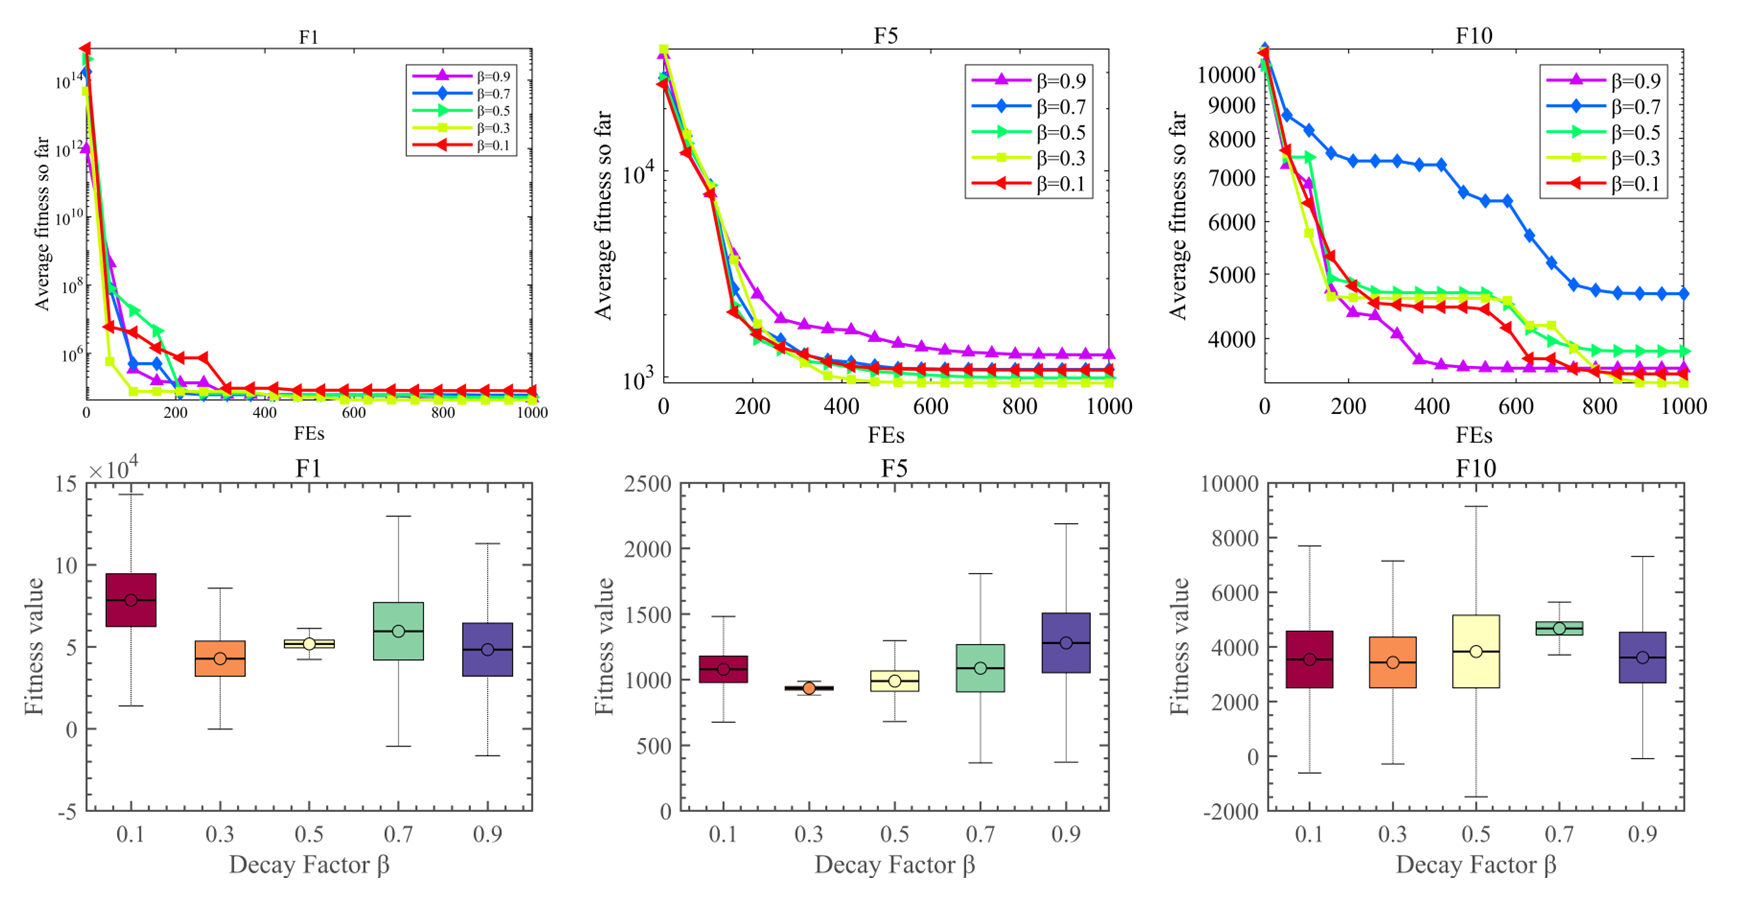
\includegraphics[width=\textwidth]{figures/chapter5/beta.png}
    \bicaption{不同$\beta$设置下BEXEA的性能}{Performance of BEXEA under different $\beta$ settings}
    \label{fig:bexea_Beta}
\end{figure}

\begin{figure}
    \centering
    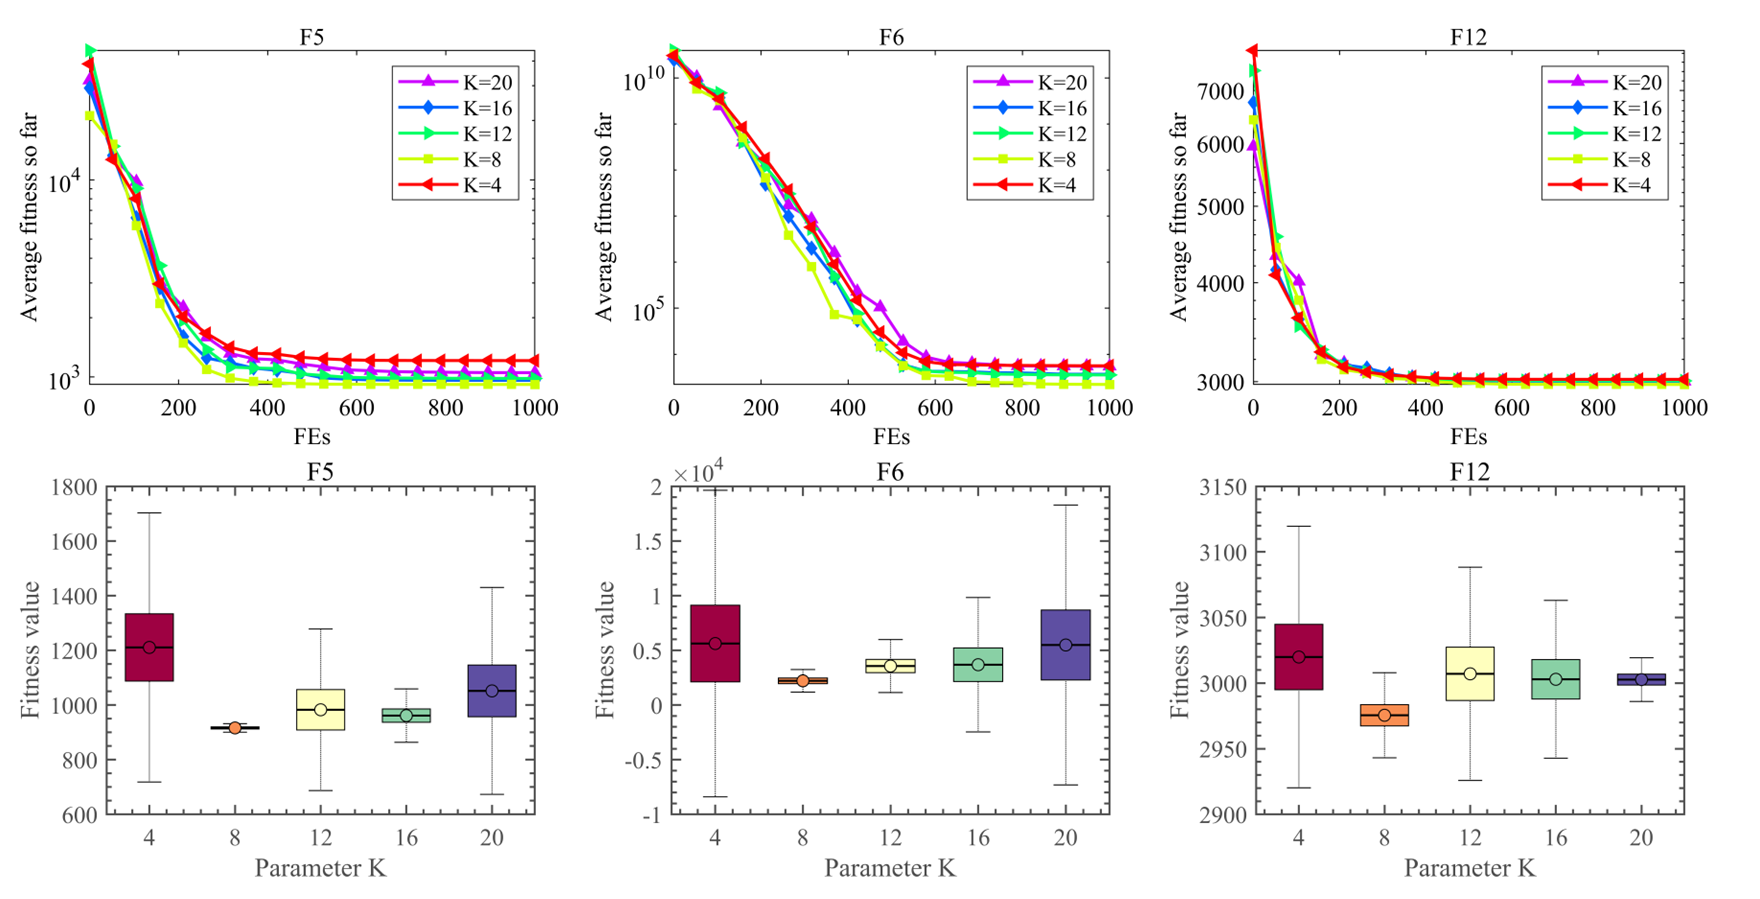
\includegraphics[width=\textwidth]{figures/chapter5/k.png}
    \bicaption{不同$\mathcal{K}$设置下BEXEA的性能}{Performance of BEXEA under different $\mathcal{K}$ settings}
    \label{fig:bexea_K}
\end{figure}

\subsubsection{油藏产量优化实验}

本项实验采用了MRST工具箱构建仿真环境，针对复杂的井控问题进行实测。

\begin{table}[htbp]
\bicaption{BEXEA与其他SAEAs在油藏产量优化问题上的比较结果}{Comparison results of BEXEA and other SAEAs on the oil reservoir production optimization problem}
\label{t:bexea_Oil_Exp_Table}
\resizebox{\textwidth}{!}{
\begin{tabular}{lcccc}
\toprule
Algorithm & Avg(std)                    & Worst             & Best              & Running time      \\
\midrule
TSABFEA   & 7.7893E+07(1.63E+05)          & 7.7567E+07          & 7.8219E+07          & 3.4710E+04          \\
KTA2      & 7.7750E+07(7.01E+05)          & 7.6348E+07          & 7.9152E+07          & 4.6481E+04          \\
DESO      & 7.6402E+07(7.53E+05)          & 7.4896E+07          & 7.7908E+07          & 2.8266E+04          \\
MS\_MTO   & 7.9145E+07(3.76E+05)          & 7.8393E+07          & 7.9897E+07          & 2.4439E+04          \\
ESA       & 7.6279E+07(6.18E+05)          & 7.5043E+07          & 7.7515E+07          & 2.5137E+04          \\
ToSADE    & 7.8500E+07(6.34E+05)          & 7.7232E+07          & 7.9768E+07          & 2.5435E+04          \\
SHPSO     & 7.6296E+07(3.42E+05)          & 7.5612E+07          & 7.6980E+07          & 2.3522E+04          \\
BEXEA     & \textbf{7.9995E+07(1.12E+05)} & \textbf{7.9771E+07} & \textbf{8.0219E+07} & \textbf{2.1334E+04}\\
\bottomrule
\end{tabular}}
\end{table}

表\ref{t:bexea_Oil_Exp_Table}的结果显示，BEXEA在所有核心经济指标上均优于竞争算法。其平均NPV不仅较次优算法提升了逾百万美元，且在结果的一致性（标准差）与运行效率方面也展现出明显优势。这种高效性对于需要频繁执行高保真模拟的石油工程决策而言，具有极高的实用价值。

\begin{figure}
    \centering
    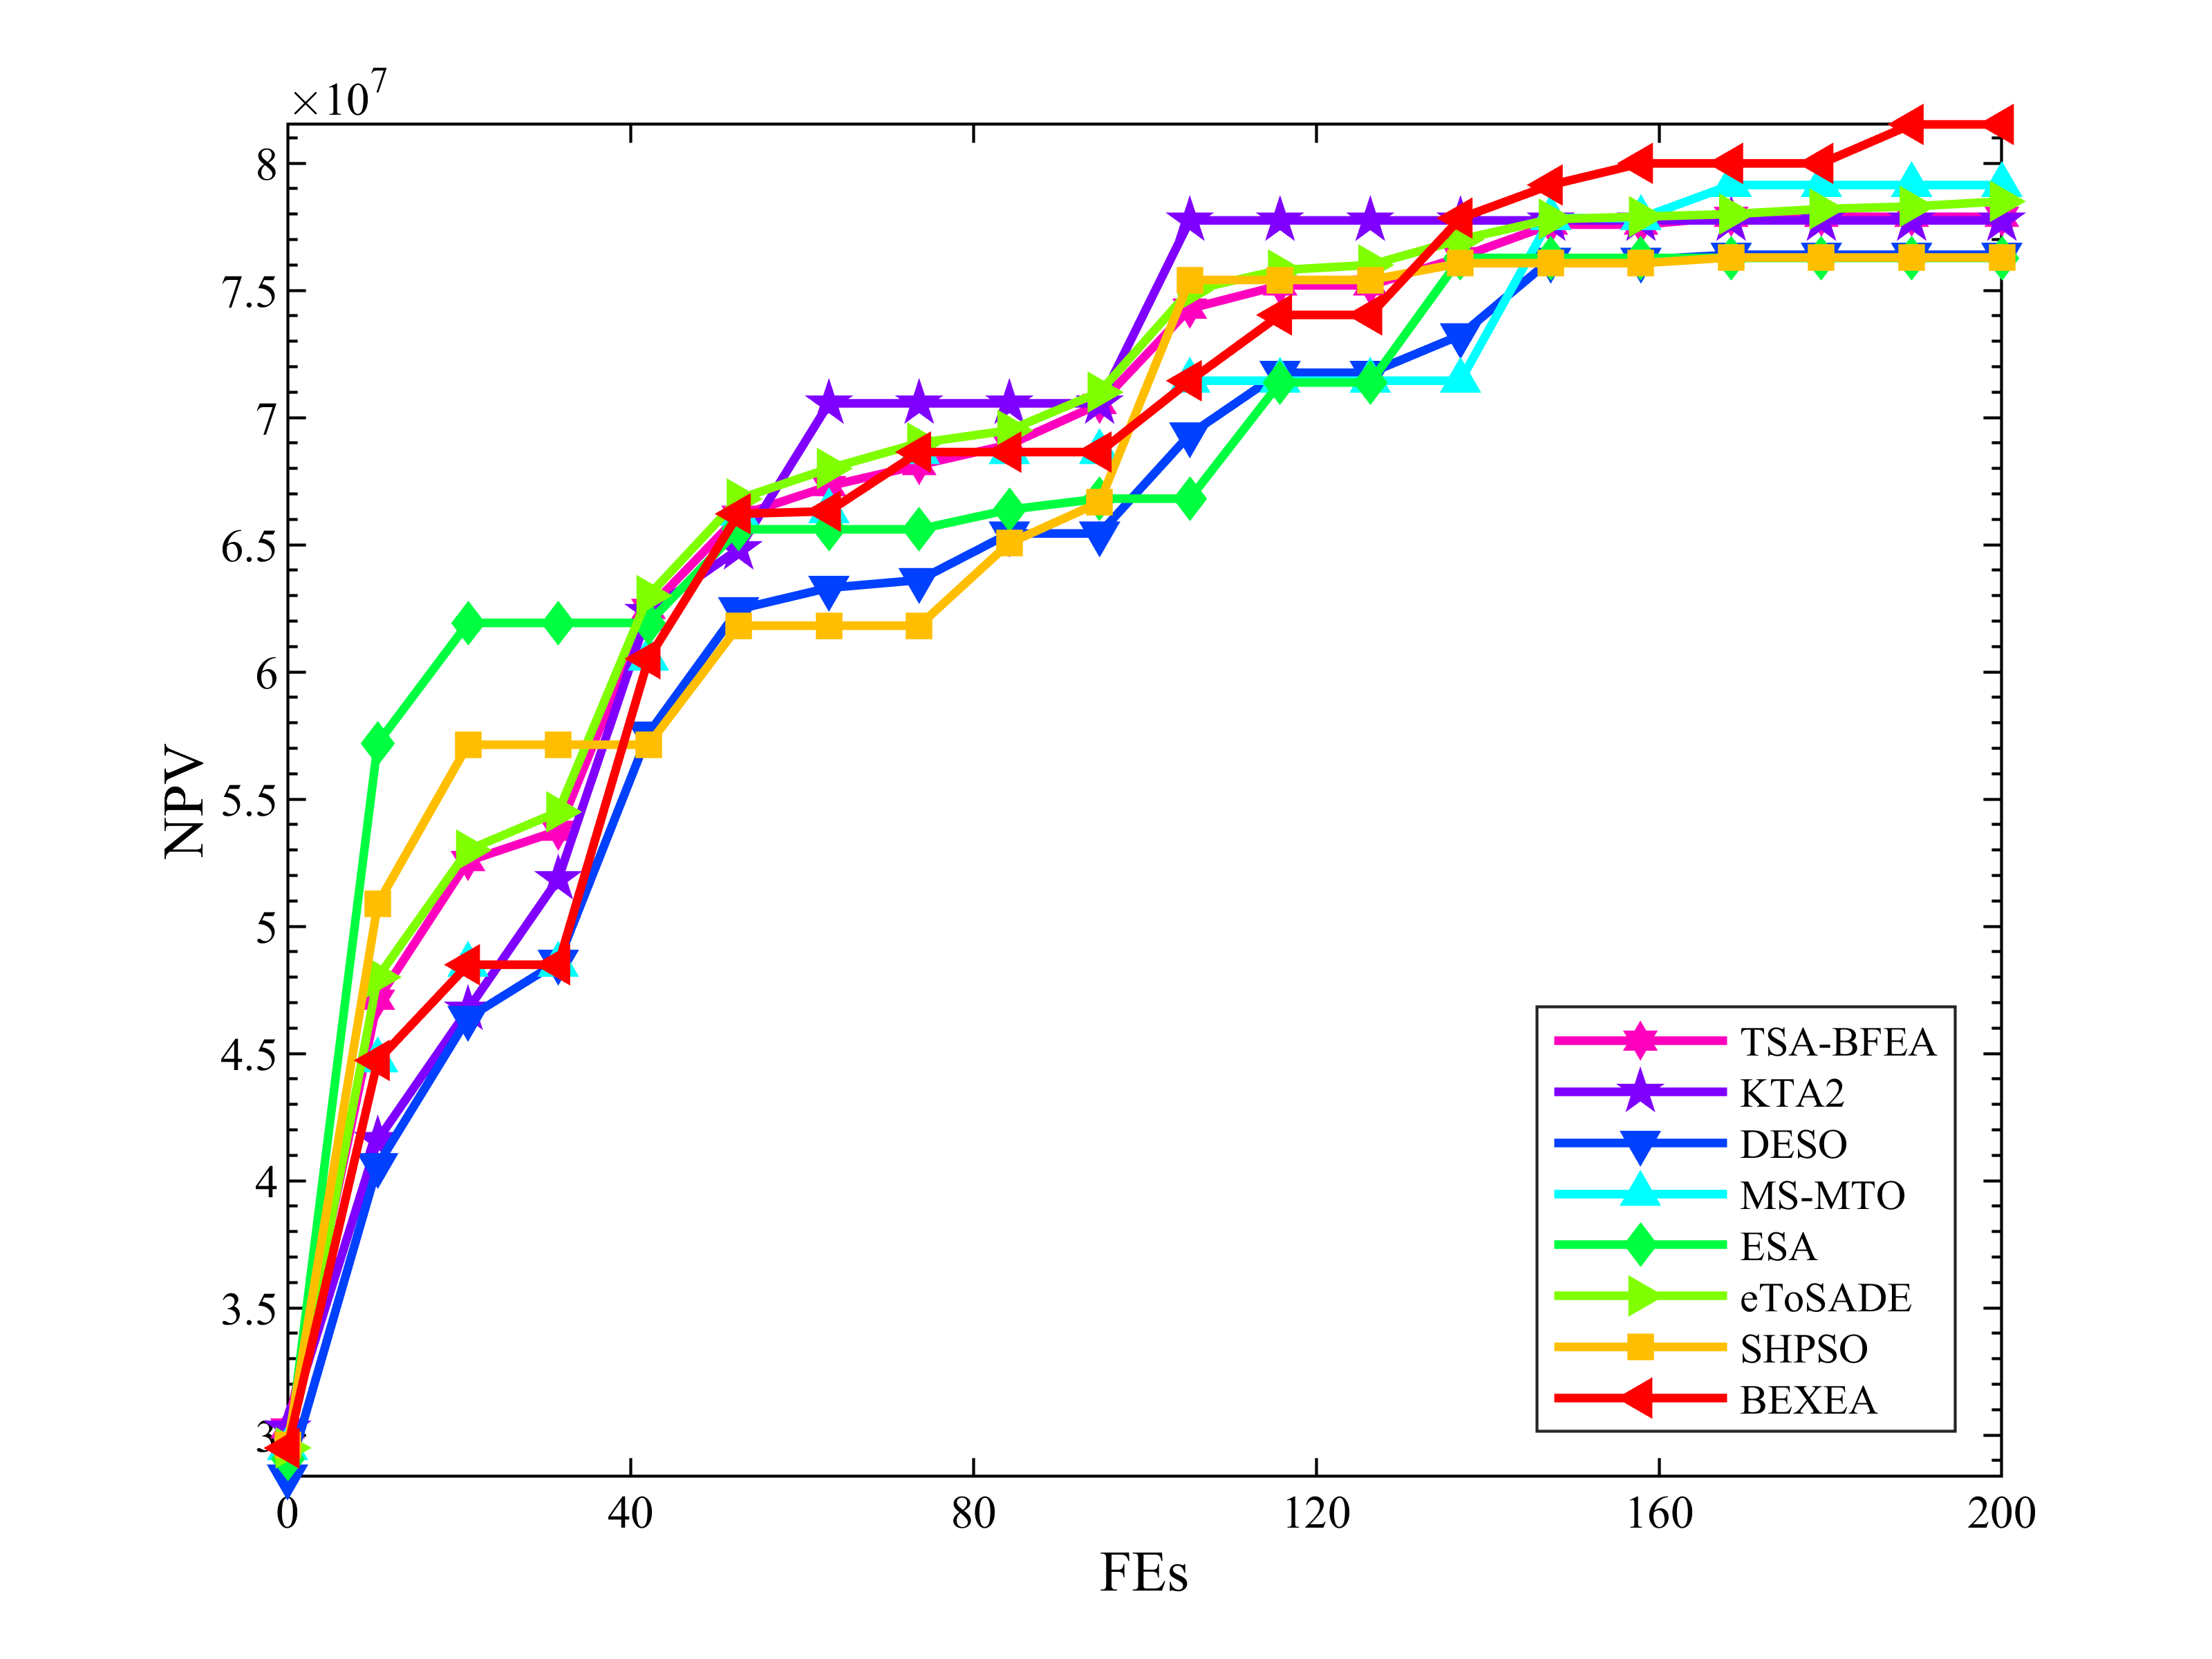
\includegraphics[width=\textwidth]{figures/chapter5/runBEXEA-OilReservoir-sampled-CC.png}
    \bicaption{BEXEA与其他SAEAs在油藏产量优化问题上的收敛曲线}{Convergence curves of BEXEA and other SAEAs on the oil reservoir production optimization problem}
    \label{fig:bexea_Oil_Exp_Figure}
\end{figure}

图\ref{fig:bexea_Oil_Exp_Figure}刻画的收敛轨迹展示了BEXEA极佳的起步能力。在优化的中后期，得益于MAB机制对搜索陷入停滞的敏锐捕捉与及时调整，算法能持续保持向更优解靠拢的势头，最终在受限的评估预算内取得了最佳经济收益。

\section{本章小结}
本章针对代理辅助昂贵优化中普遍存在的策略僵化与采样准则黑箱化问题，研发了BEXEA算法。该方法通过融合多臂赌博机的自适应搜索与可解释人工智能技术，实现了对搜索资源与采样决策的智能化协同管理。

全方位的实验验证表明，BEXEA在不同维度的标准测试套件上均展现了超越同类先进算法的优化能力。其在油藏工程实测算例中的成功应用，进一步印证了该方法在处理真实复杂昂贵问题时的优越样本效率与实战价值。消融实验的数据也充分解构了自适应切换与多准则采样对算法性能提升的具体贡献。整体而言，BEXEA在减少对人工先验设计依赖的同时，提升了优化决策的透明度，为昂贵优化问题的求解提供了一种更高效且具解释性的新路径。
